%\documentclass[12pt,a4paper]{article}
\documentclass[german,bibnum,beleg,zihtitle,german,hyperref,utf8]{zihpub}
\author{Maximilian Knespel}
\betreuer{Dipl.-Inf. Nico Hoffmann}
\title{Belegarbeit Computational Science and Engineering\\
       Verteilte GPGPU-Berechnungen mit Spark}
%\date{}
\bibfiles{literatur}

\usepackage[german,onelanguage]{algorithm2e}

\usepackage[utf8]{inputenc}
\usepackage[T1]{fontenc}
	% if you don't use \usepackage[T1]{fontenc},
    % - Words containing accented characters (ö,...) cannot be automatically hyphenated,
    % - You cannot properly copy-and-paste srom the output (DVI/PS/PDF),
    % - Characters like the pipe sign, less than and greater sign give unexpected results in text.
\usepackage{lmodern}  % Vector Fonts even when using T1 !
%\usepackage[ngerman]{babel}
\usepackage[dvipsnames,cmyk,table]{xcolor} % xcolor and more colornames, cymk for printing
\usepackage{cmap} % pro­vides char­ac­ter map ta­bles, which makes PDFs search­able and copy-able (I don't see a difference yet!!!)
\usepackage[labelfont=bf,format=plain]{caption} % allows captions in non-figure environments with \captionof and \captionsetup
\usepackage[binary-units=true]{siunitx}    % SI units paper conform with \SI{3}{\nano\seconds}
\usepackage{tabularx}
\newcolumntype{Y}{>{\centering\arraybackslash}X}

\definecolor{mygreen}{rgb}{0,0.6,0}
\definecolor{mygray}{rgb}{0.5,0.5,0.5}
\definecolor{mymauve}{rgb}{0.58,0,0.82}

\usepackage{listings}   % source code listings
\usepackage{textcomp}
\usepackage{courier}
\usepackage{float}      % enables \begin{figure}[H] to disable floating figure
\usepackage{ulem}

\lstset{ %
  backgroundcolor=\color{white},   % choose the background color; you must add \usepackage{color} or \usepackage{xcolor}
  basicstyle=\footnotesize\ttfamily, % the size of the fonts that are used for the code
  breakatwhitespace=false,         % sets if automatic breaks should only happen at whitespace
  breaklines=true,                 % sets automatic line breaking
  captionpos=b,                    % sets the caption-position to bottom
  commentstyle=\color{mygreen},    % comment style
%  deletekeywords={...},            % if you want to delete keywords from the given language
  escapeinside={\%*}{*)},          % if you want to add LaTeX within your code
  extendedchars=false,              % lets you use non-ASCII characters; for 8-bits encodings only, does not work with UTF-8
  %frame=single,                    % adds a frame around the code
  keepspaces=true,                 % keeps spaces in text, useful for keeping indentation of code (possibly needs columns=flexible)
  keywordstyle=\color{blue},       % keyword style
  morekeywords={*,...},            % if you want to add more keywords to the set
  numbers=left,                    % where to put the line-numbers; possible values are (none, left, right)
  numbersep=5pt,                   % how far the line-numbers are from the code
  numberstyle=\tiny\color{mygray}, % the style that is used for the line-numbers
  rulecolor=\color{black},         % if not set, the frame-color may be changed on line-breaks within not-black text (e.g. comments (green here))
  showspaces=false,                % show spaces everywhere adding particular underscores; it overrides 'showstringspaces'
  showstringspaces=false,          % underline spaces within strings only
  showtabs=false,                  % show tabs within strings adding particular underscores
  stepnumber=1,                    % the step between two line-numbers. If it's 1, each line will be numbered
  stringstyle=\color{mymauve},     % string literal style
  tabsize=2,                       % sets default tabsize to 2 spaces
  title=\lstname,                  % show the filename of files included with \lstinputlisting; also try caption instead of title
  xleftmargin=.25in,               % indent listings by default
  upquote=true                     % single quotes '' appear straight instead of as backticks. Needs textcomp
}

\usepackage{amsmath, amsthm, amssymb}
\allowdisplaybreaks
\setlength\parindent{0pt} % stop indenting every paragraph by 1cm. It looks awful!
\usepackage{esint} % for oiint
\usepackage{attachfile} % insert attachments into pdf O_O

%\usepackage{pdfpages}   % include single pages from larger pdfs (this is a pdfxcviewerpro feature, it's cool that latex can do this for free!!)

\usepackage{enumitem}
\setitemize{itemsep=0pt,topsep=3pt}
\setenumerate{itemsep=0pt,topsep=3pt}

% http://tex.stackexchange.com/questions/2644/how-to-prevent-a-page-break-before-an-itemize-list
\makeatletter
\newcommand{\nolisttopbreak}{\vspace{\topsep}\nobreak\@afterheading}
\makeatother

\addto\extrasngerman{\def\figureautorefname{Abb.}} % for use with autoref
\addto\extrasngerman{\def\equationautorefname{Gl.}} 
\addto\extrasngerman{\def\sectionautorefname{Kapitel}} 
\addto\extrasngerman{\def\subsectionautorefname{Kapitel}} 
\addto\extrasngerman{\def\subsubsectionautorefname{Kapitel}} 

%%%%%%%%%%%%%%%%%%%%%%%%%%%%%%%%%%%%%%%%%%%%%%%%%%%%%%%%%%%%%%%%%%%%%%%%%%%%%%%%
% main part
%%%%%%%%%%%%%%%%%%%%%%%%%%%%%%%%%%%%%%%%%%%%%%%%%%%%%%%%%%%%%%%%%%%%%%%%%%%%%%%%

\begin{document}

\hyphenchar\font=\string"7F % make "= unneeded
%\hyphenation{Kon-fi-gu-ra-ti-ons-tool} % why isn't this working damn it!?

% All files must be UTF8-without BOM encoded!!!

%sed -e 's/\\section/\\chapter/'          -i Aufgabe*.tex
%sed -e 's/\\subsection/\\section/'       -i Aufgabe*.tex
%sed -e 's/\\subsubsection/\\subsection/' -i Aufgabe*.tex

\chapter{Einführung}
Im Rahmen dieser Belegarbeit soll ein Ansatz entwickelt werden, um in Java oder Scala auf Clustern auf Grafikkarten zu berechnen. Es wurde sich für eine Kombination von Spark für die Kommunikation im Cluster und Rootbeer für die Grafikkartenprogrammierung entschieden.

Zuerst wird in den Kapiteln \ref{sct:montecarloalgo}-\ref{sct:spark} die benutzten Algorithmen und Bibliotheken vorgestellt, in Kapitel~\ref{sct:implementation} wird die eigene Implementierung dokumentiert und in Kapitel~\ref{sct:benchmarks} werden Benchmarks dieser Implementierung vorgestellt.

%Dabei soll die Vorgehensweise reproduzierbar dokumentiert werden, mit dem Ziel, die Programmierung auf Grafikkarten-Clustern so einfach wie möglich zu machen. Z.B. durch ein Skript. Als ersten Testfall wird ein Monte-Carlo-Algorithmus zur Berechnung von Pi implementiert, da dieser sehr rechenlastig ist. Weiterhin soll ein kommunikationslastiger Algorithmus wie z.B. Mergesort auf einem Grafikkartencluster untersucht werden.

\chapter{Rechenintensiver Testalgorithmus}
\label{sct:montecarloalgo}

\section{Monte-Carlo Algorithmen}

Monte-Carlo-Algorithmen bezeichnet Algorithmen, die mit Hilfe von (Pseudo-)Zufallszahlen versuchen das gesuchte Ergebnis statistisch zu approximieren. Dafür werden Stichproben aus statistischen Verteilungen durch z.B. physkalisch begründete Abbildungen transformiert und jene Ergebnisse statistisch ausgewertet. Diese Art von Verfahren eignet sich z.B. zur Berechnung von Integralen über zig Koordinaten, die mit üblichen Newton-Cotes-Formeln aufgrund der hohen Dimensionalität nicht praktikabel wären. Eine andere Anwendung ist die Analyse von durch kosmischer Strahlung ausgelösten Teilchenschauern mit Hilfe von Markov-Ketten\cite{metropolis1949monte}.

Monte-Carlo-Algorithmen sind als statistische Stichprobenverfahren schon länger bekannt, wurden aber erst mit dem Aufkommen der ersten Computer, z.B. dem ENIAC um 1947-1949, praktikabel\cite{metropolis1987beginning}. Der Name, nach der Spielbank ''Monte-Carlo'', wurde von N.Metropolis vorgeschlagen und hielt sich seitdem. Der Vorschlag zu dieser Art von Algorithmus kam von John von Neumann auf, als man mit dem ENIAC thermonukleare Reaktionen simulieren wollte. Aber Fermi wird nachgesagt schon Jahre zuvor statistische Stichprobenverfahren in schaflosen Nächten händisch angewandt zu haben und mit den überraschend genauen Resultaten seine Kollegen in Staunen zu versetzen.

Monte-Carlo-Verfahren sind inhärent leicht zu parallelisieren, da eine Operation, die Simulation, mehrere Tausend oder Milliarden Mal ausgeführt wird. Eine Schwierigkeit besteht jedoch darin den Pseudozufallszahlengenerator (pseudorandom number generator - PRNG) korrekt zu parallelisieren. Das heißt vor allem muss man unabhängige Startwerte finden und an die parallelen Prozesse verteilen.
 - Zeitangaben sind hierbei nicht sinnvoll. Das betrifft alle möglichen Zeitgeber in Rechnern wie z.B. .

\subsection{Berechnung von Pi}

Um Pi zu berechnen wird Pi als Integral dargestellt, da sich beschränkte Integrale durch Monte-Carlo-Verfahren approximieren lassen.
\begin{equation}
	\pi = \int \begin{cases}
					1 & |x^2+y^2| \leq 1\\
					0 & \text{sonst}
			   \end{cases}
		  \mathrm{d}x \mathrm{d}y
\end{equation}
Das heißt wir integrieren die Fläche eines Einheitskreises. Durch die Ungleichung wissen wir auch, dass nur für $x,y\in [-1,1]$ der Integrand ungleich $0$ ist.

Da es programmatisch trivialer ist Zufallszahlen aus dem Intervall $[0,1]$ anstatt $[-1,1]$ zu ziehen, wird das Integral über den Einheitskreis in ein Integral über einen Viertelkreis geändert:
\begin{equation}
	\label{eq:piint}
	\pi = 4 \int\limits_{0}^\infty \mathrm{d}x
		    \int\limits_{0}^\infty \mathrm{d}y
		    \begin{cases}1 & |x^2+y^2| \leq 1\\0 & \text{sonst} \end{cases}
\end{equation}

Das Vorgehen ist nun wie folgt
\begin{enumerate}
	\item Setze die Zählvariable \texttt{Summe} auf $0$
	\item Ziehe für $x$ und $y$ je eine gleichverteilte Zufallszahl aus dem Intervall $[0,1]$\
	\item Falls $x^2+y^2<1$, dann erhöhe \texttt{Summe} um $1$
	\item Gehe zu 2.
\end{enumerate}
Mathematisch ausgedrückt also:
\begin{equation}
	\label{eq:pimonteint}
	\mu_N = \langle f\left( \vec{x}_i \right) \rangle := \frac{1}{N} \sum_{i=1}^N f\left( \vec{x}_i \right),\;\vec{x}_i \text{ uniform zufallsverteilt aus } \Omega:=[0,1]\times[0,1]
\end{equation}
Im allgemein ist $f$ eine beliebige Funktion, aber für die Berechnung von Pi ist es die Einheitskugel in 2D, vgl.Gl.\ref{eq:piint}.

In Python kann man dies, wenn man sich auf Einkernprozessoren einschränkt, mit NumPy\cite{numpy} in nur wenigen zeilen niederschreiben:
\begin{lstlisting}[language=python]
from numpy import *
N=10000000
x=random.rand(N)
y=random.rand(N)
pi = 4.0 * sum( x*x + y*y < 1 ) / N
\end{lstlisting}\vspace{-1.5\baselineskip}

Der Vollständigkeit halber seien kurz ein paar Worte zu den Rändern verloren, das betrifft die Zufallszahlen die entweder aus einem rechtsoffenem oder geschlossenen Intervall $[0,1]$ stammen können und den Vergleich, der die Gleichheit mit einschließen kann oder nicht.

Aus der Integraltheorie ist klar, dass die Ränder ein Nullmaß haben und damit keine Rolle spielen. Aber für diskrete Verfahren könnte dies zu einer zusätzlichen systematischen Fehlerquelle führen, der Fehlerskalierverhalten möglicherweise beeinträchtigt.

Am Beispiel von nur vier Zuständen für Zufallszahlen für den rechtsoffenen Fall, also $x,y\in \lbrace 0,0.25,0.5,0.75 \rbrace$, sei dies einmal durchgedacht. Damit ergibt sich
\begin{equation}
	x^2+y^2 = \lbrace 0, 0.0625, 0.125, 0.25, 0.3125, 0.5, 0.5625, 0.625, 0.8125, 1.125 \rbrace
\end{equation}
% (Python-Skript für Kombinationen:
%    x=array([0,1,2,3])/4.
%    a,b=meshgrid(x**2,x**2)
%    unique( (a+b).ravel() )
Hier macht es aufgrund der begrenzten Anzahl an Zuständen, unter denen die $1.0$ ohnehin nicht auftritt, keinen Unterschied ob man $<$ oder $\leq$ vergleicht, man erhielte Pi zu $3.6$.
Hinzu kommt aber, dass Zustände auf den Grenzen $x=0$ und $y=0$ liegen, sodass die Grenzen vierfach gezählt werden da wir nur den Viertelkreis berechnen und mit vier multiplizieren.

Man hat also ohnehin immer einen Diskretisierungsfehler von $O\Delta x)$ wobei $\Delta x$ die Diskretisierungslänge zwischen zwei Zuständen ist. Angemerkt sei, dass dies für Gleitkommazahlen komplizierter gestaltet.

Abschließend sei angemerkt, dass Monte-Carlo-Methoden dafür gedacht sind einen praktisch unerschöpflichen Raum Stichprobenartig auszutesten, sodass Diskretisierungs- und Randfehler ohnehin als vernachlässigbar angenommen werden. Wenn man merkt, dass es zu Diskretisierungsfehler wie obig an den Rändern kommt, oder man gar die Anzahl aller möglichen Zustände an Zufallszahlen erschöpft hat und sich die Approximation damit nicht mehr verbessern kann, sollte man über ein anderes Verfahren nachdenken oder den Zufallsgenerator anpassen und z.B. mit 128-Bit statt 32-Bit betreiben. Auch die maximale Periodenlänge von Pseudozufallsgeneratoren spielt hier eine Rolle!
%
%Mit geschlossenen Grenzen hingegen wären $x,y\in\lbrace 0,\frac{1}{3},\frac{2}{3},1 \Rightarrow \rbrace 0, \frac{1}{9}, \frac{2}{9}, \frac{4}{9}, \frac{5}{9}, \frac{8}{9}, 1 \frac{10}{9}, \frac{13}{9},2 \rbrace$
% Man beachte, dass float ohnehin nur 32 Bit ist, wovon 1 bit das Vorzeichen und 8 bit der Exponent ist. Da wir uns immer nur im Intervall [0,1] befinden nutzen wir Vorzeichen und Exponent ohnehin nicht, sodass nur 23 Bit Präzision benutzt werden. Das sind also nur 2^23 \approx 10^7 erreichbare Zustände. Moderne Prozessoren können leicht 10^9 Operationen pro Sekunde rechnen, sodass einfache Fließkommagenauigkeit nicht ausreicht, da schon nach einigen Millionen Stichproben sich der relative Fehler nicht mehr verbessern, aber auch nciht mehr verschlechtern, wird. Siehe dazu Abb.\ref{fig:monteerrorfloat}

Da die Monte-Carlo-Pi-Integration einer Mittelwertbildung entspricht, vgl. Gl.\ref{eq:pimonteint}, ist die statistische Unsicherheit gegeben durch die Standardabweichung des Mittelwerts $\sigma_{\mu_N}$, welche gegeben ist als
\begin{equation}
	\sigma_{\mu_N} \frac{\sigma}{\sqrt{N}}
\end{equation}
wobei $\sigma$ die Standardabweichung der Stichprobe ist, vgl. Anhang~\ref{apx:meanerror}.
Wenn $f_i$ in einem beschränkten Intervall liegt, dann ist auch die Standardabweichung der Stichproben $f_i$ beschränkt, sodass die Standardabweichung auf den Mittelwert $\propto \frac{1}{\sqrt{N}}$ abnimmt.

\begin{figure}
	\centering
	\begin{minipage}{0.7\linewidth}
		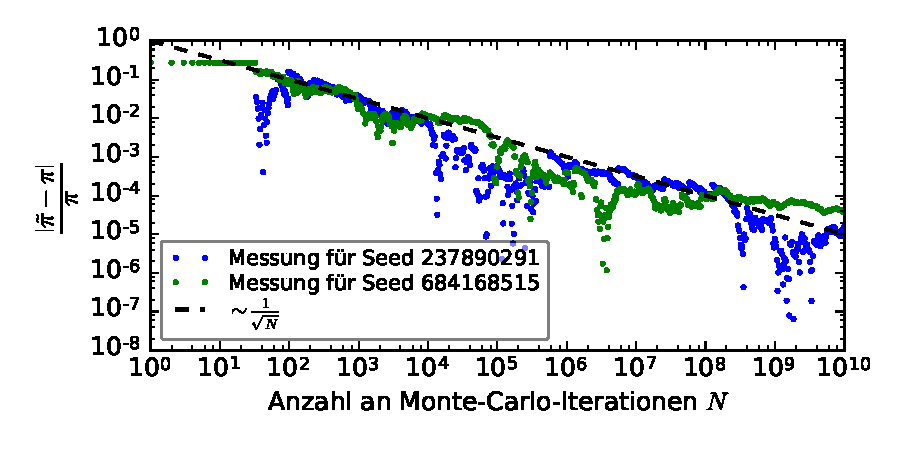
\includegraphics[width=\linewidth]{monte-carlo-pi-error-scaling}
	\end{minipage}
	\caption{captiontext}
	\label{fig:monteerrorfloat}
\end{figure}


%\subsection{Pseudozufallszahlgeneratoren}
%\section{Vergleich - Alternativen}


%%%%%%%%%%%%%%%%%%%%%%%%%%%%%%%%%%%%%%%%%%%%%%%%%%%%%%%%%%%%%%%%%%%%%%%%%%%%%%%%
\chapter{Apache Spark}
\label{sct:spark}
%%%%%%%%%%%%%%%%%%%%%%%%%%%%%%%%%%%%%%%%%%%%%%%%%%%%%%%%%%%%%%%%%%%%%%%%%%%%%%%%

Spark ist ein Programmierframework für Datenanalyse auf Clustern, was vor allemim Zusammenhang mit ''Big Data'' an Beliebtheit gewonnen hat.
Es vereinigt hierbei ausfallgehärtet Funktionalitäten von Batchverarbeitungssystemen bzw. Cluster-Management wie z.B. SLURM, Kommunikation zwischen Prozessen, wie z.B. OpenMPI und OpenMP sie zur Verfügung stellen, und zusätzliche problemspezifische Programmierbibliotheken.
Spark stellt Programmierschnittstellen für Java, Scala und Python zur Verfügung. Für Scala und Python existieren interaktive Eingabeaufforderungen mit der z.B. interaktive Echtzeitanalysen auf Clustern mit Spark möglich sind.\\

Apache Spark oder auch Spark Core stellt die Grundfunktionalität für verteiltes Rechnen bereit.
Das inkludiert die erwähnte Ausfallsicherheit, Management von Knoten über ein Web-Interface und Prozess-Scheduling\cite{learningspark}.
Die Programmierschnittstelle hierfür sind der Spark-Kontext und die Resilient Distributed Datasets (RDD).

\begin{figure}
    \centerline{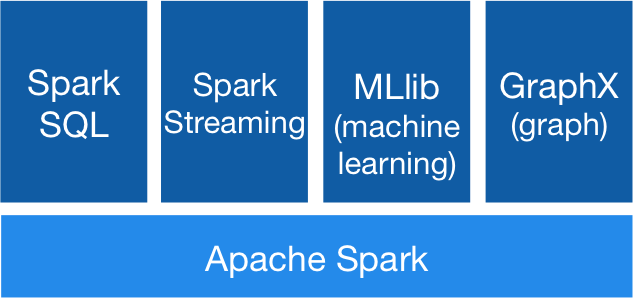
\includegraphics[width=0.5\linewidth]{spark-stack.png}}
    \caption{Zusammensetzung des Spark-Frameworks\cite{spark}}
    \label{fig:sparkstack}
\end{figure}

Beispielhaft für den Spark-Stack seien hier die Bibliotheken MLlib\cite{mllib} und GraphX erwähnt.

MLlib, kurz für Machine Learning Library, umfasst Funktionen wie lineare Regression, den K-Means-Algorithmus, Latent Dirichlet Allocation, Hauptkomponentenanalyse, das für Maschinenlernen benötigte stochastische Gradientenverfahren, u.v.m.

% GraphX
GraphX erweitert Spark-RDDs zu Kanten- und Knoten-RDDs die als Tupel einen Graph beschreiben \cite{graphx}. Auf diesen abgeleiteten Datentypen sind übliche RDD- und Mengenoperationen wie \lstinline!subgraph!, \lstinline!diff!, u.a. für das Erstellen und Modifizieren von Graphen möglich.
Ein solcher Graph kann z.B. Webseitenrelationen, jeder Link ist eine Kante im Graph, jede Domain ein Knoten, darstellen.
Auf diesen Graphen sind Algorithmen wie PageRank oder das Auszählen von Dreiecken in Graphen ausführbar.

%%%%%%%%%%%%%%%%%%%%%
\section{MapReduce}
%%%%%%%%%%%%%%%%%%%%%

Spark basiert auf dem MapReduce-Paradigma, welches 2004 in einem Paper der Google-Mitarbeiter Dean und Ghemawat\cite{mapreduce2004,mapreduce2008} in Anlehnung an die aus funktionalen Programmiersprachen bekannten Map- und Reduce-Befehle eingeführt wurden.
Viele der benötigten Algorithmen wie Häufigkeitsanalyse oder Webseitengraphen hatten zuvor ihren eigenen Programmcode für die Kommunikation und Ausfallsicherheit im Cluster und folgten von der Struktur her einem simplem Schema: zuerst werden Eingabedaten datenparallel verarbeitet und anschließend werden die Zwischenergebnisse zu Endergebnissen reduziert.
Diese einfach gestrickten Algorithmen mussten aber trotzdem auf beträchtlichen Datenmengen auf Knoten hoher Ausfallwahrscheinlichkeit laufen. Diese Funktionalität, also die Kommunikation im Cluster und die Ausfallsicherheit. wurde so in eine MapReduce-Bibliothek ausgelagert.

MapReduce bezeichnet hierbei sowohl das Programmierparadigma als auch die Bibliothek, die diese ausfallsicher und parallelisiert zur Verfügung stellt.
Dafür definiert der Nutzer eine Map-Funktion die aus einer Liste jedes Schlüssel-Wert-Paar $(k,v)$ auf eine Liste aus neuen Schlüssel-Wert-Paaren abbildet:
\begin{equation}
    \mathbf{Map : }\left( k, v \right) \mapsto
    \left[ \left( l_1, x_1 \right), \ldots, \left( l_{r_k}, x_{r_k} \right) \right]
\end{equation}
$k$ und $l$ sind hierbei die Schlüssel und $v$ und $x$ die dazugehörigen Werte. Für $r_k=1$ erhält man den Grenzfall, dass jeder Schlüssel-Wert-Tupel auf exakt einen neuen Schlüssel-Wert-Tupel abgebildet wird.

Da es per Definition keine Abhängigkeiten zu anderen Schlüssel-Wert-Paaren für die Berechnung der Map-Funktion gibt, kann jedes Datum parallel berechnet werden.
Das MapReduce-Framework stellt außerdem Funktionen zum Einlesen von Daten zur Verfügung und verteilt diese automatisch an die Knoten des Clusters, wo diese dann parallel verarbeitet werden.

In einem impliziten Schuffle-Schritt werden alle Paare mit gleichem Schlüssel lokal gruppiert, d.h. es werden alle Paare z.B. mit Schlüssel $k_1=\mathrm{'Dresden'}$ auf dem gleichen Knoten im Cluster gesammelt.
Dieser Schritt kann also sehr kommunikationsaufwendig sein.
Der Nutzer kann nur über die Art der Schlüssel auf diesen Prozess Einfluss nehmen.
Man erhält als Ergebnis des Schuffle-Schritts einen Tupel aus einem Schlüssel und einer Liste an dazugehörigen Werten.
\begin{equation}
    \mathbf{Shuffle :}
    \left[ \left( k_1, x_1 \right), \ldots, \left( k_n, x_n \right) \right]
    \mapsto \left[ \left( l_1, \left[ y^1_1, \ldots, y^1_{r_1} \right] \right), \ldots,
    \left( l_m, \left[ y^m_1, \ldots, y^m_{r_m}) \right] \right) \right]
\end{equation}

Im nachfolgenden Reduce Schritt werden die Tupel aus Schlüssel und Werteliste mit einer vom Nutzer defineirten Reduce-Funktion abgebildet auf eine neue Werteliste.
Im einfachsten Fall kann die neue Werteliste nur ein Element enthalten, z.B. die Summe oder den Mittelwert der alten Werte.
\begin{equation}
    \mathbf{Reduce : }
    \left( l, \left[ y_1, \ldots, y_{s_l} \right] \right)
    \mapsto \left[ w_1, \ldots, w_{m_l} \right]
\end{equation}

Auch die Reduce-Operation kann also bezüglich einzigartiger Schlüssel datenparallel ausgeführt werden.
Anfangs war dieses Paradigma nur für einfache Beispiele wie Wortfrequenzanalysen gedacht, aber mittlerweile wurden auch komplexere Algorithmen wie z.B. Matrixmultiplikation\cite{matmulmapreduce} oder das Problem des Finden einer maximalen Überdeckung\cite{maxcovermapreduce} ins MapReduce-Schema portiert.\\

%%%%%%%%%%%%%%%%%%%%%
% MapReduce
%%%%%%%%%%%%%%%%%%%%%

Eine lange Zeit beliebte Implementation basierend auf dem MapReduce-Paper\cite{mapreduce2004} ist Apache Hadoop\cite{hadoop}.
Hadoop besteht aus einem verteilten Dateisystem, dem Hadoop Distributed File System (HDFS), und einer Bibliothek namens MapReduce, die Funktionen für das Rechnen auf den verteilten Daten anbietet.

Apache Spark\cite{spark} ist eine alternative Implementation des MapReduce-Modells.
Es versucht viele der Probleme von Hadoop zu beheben, bietet jedoch neben dem Zugriff vom lokalen Dateisystem auch den Zugriff von HDFS und weiteren verteilten Dateisystemen aus an.

Einer der Hauptvorteile von Spark ist der Geschwindigkeitsgewinn bei der iterativen Anwendung von Map und Reduce durch die Möglichkeit die Daten auch im Arbeitsspeicher, nicht nur auf der Festplatte, der Knoten zwischenzuspeichern.


%%%%%%%%%%%%%%%%%%%%%%%%%%%%%%%%%%%%%%%%%%%%%%%%%%%%%%%%%%%%%%%%%%%%%%%%%%%%%%%%
\section{Architektur}
%%%%%%%%%%%%%%%%%%%%%%%%%%%%%%%%%%%%%%%%%%%%%%%%%%%%%%%%%%%%%%%%%%%%%%%%%%%%%%%%

% Executor, Masternode
Für kleinere Tests kann Spark local auf einem Computer bzw. Knoten ausgeführt werden:
\begin{lstlisting}[numbers=none]
spark-shell --master local[*]
\end{lstlisting}\vspace{-1.5\baselineskip}
In diesem Beispielaufruf der interaktiven Spark-Shell werden so viele Threads genutzt wie es logische Kerne gibt.

Für das Ausführen auf einem Cluster ist jedoch das getrennte Starten von einem Spark Driver (Master) und mindestens einem Executor (Slave, Worker) notwendig, vgl. \autoref{fig:sparkcluster}.
Der Spark-Driver führt das geschriebene Spark-Programm aus und verteilt u.a. die für die Map-Funktion benötigten Daten an die Executoren, welche die zugewiesenen Berechnungen dann durchführen.

\begin{figure}
    \centerline{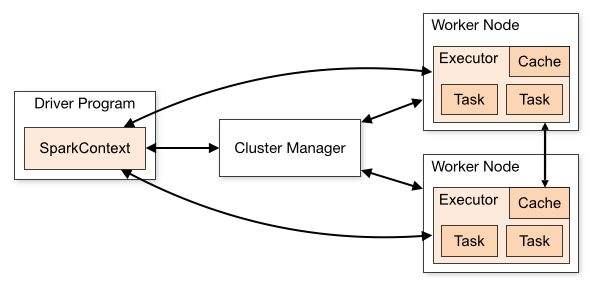
\includegraphics[width=0.8\linewidth]{cluster-overview.png}}
    \caption{Master/Slave-Struktur eines Spark-Clusters\cite{spark}}
    \label{fig:sparkcluster}
\end{figure}

Jeder Executor wird in einer eigenen Java Virtual Machine (JVM), also einem eigenen Prozess ausgeführt.
Normalerweise, und so auch hier, wird für jeden Knoten ein Executor-Prozess gestartet, welcher mit der in der \lstinline!SPARK_WORKER_CORES!-Umgebungsvariable definierten Anzahl an Threads arbeitet.
Für den hier vorgestellten Benchmark wird \lstinline!$SPARK_WORKER_CORES! identisch der Anzahl an Grafikkarten auf dem Knoten gewählt, sodass jeder Thread mit genau einer Grafikkarte arbeitet.\\

Ein RDD kann z.B. mit \lstinline!parallelize! erstellt werden \cite{sparkguide}.
\begin{lstlisting}[numbers=none,language=scala]
val distData = sc.parallelize( 1 to 10, 5 )
\end{lstlisting}\vspace{-1.5\baselineskip}
In diesem Beispiel wurden die Zahlen 1 bis 10 in ein RDD geladen.
Das zweite Argument gibt die Anzahl an Partitionen an, die das RDD nutzen soll.
Hier werden die Daten also in 5 Partitionen, in älteren Versionen von Spark auch Slices genannt, aufgeteilt.
Eine Partition ist wie ein Task zu verstehen, der von einem der Executoren ausgeführt wird.
Die Anzahl an Partitionen gibt damit eine Obergrenze für die Parallelisierbarkeit vor.
Um Gebrauch von einer optimalen Lastverteilung zu machen sollte man eine Größenordnung mehr Partitionen haben, als die Sparkinstanz logische Kerne bzw. Threads zur Verfügung hat.


%%%%%%%%%%%%%%%%%%%%%%%%%%%%%%%%%%%%%%%%%%%%%%%%%%%%%%%%%%%%%%%%%%%%%%%%%%%%%%%%
\section{Konfiguration von Spark auf einem Slurm-Cluster}
\label{sct:sparkconfig}
%%%%%%%%%%%%%%%%%%%%%%%%%%%%%%%%%%%%%%%%%%%%%%%%%%%%%%%%%%%%%%%%%%%%%%%%%%%%%%%%

Viele Cluster stellen schon einen Task-Scheduler für Multinutzerumgebungen, wie z.B. PBS (Portable Batch System) oder SLURM (Simple Linux Utility for Resource Management), zur Verfügung, um Rechenzeit auf dem Cluster möglichst effizient und gerecht zu verteilen.
Außerdem ermöglichen sie das verteilte Starten von Programmen, z.B. jene die mit MPI programmiert wurden.
Der für die Benchmarks genutzte Cluster, siehe \autoref{sct:taurus}, arbeitet mit SLURM.\\

Um Spark nutzen zu können, müssen zuerst Master- und Slave-Knoten gestartet werden.
Damit alle gleichzeitig gestartet werden, sollten sie innerhalb desselben Jobs initiiert werden.
Dies kann z.B. mit SLURMs \lstinline!--multi-prog! Option realisiert werden. Der Pfad zu der ausführbaren Datei wird dann als Konfigurationsdatei interpretiert, in der für jeden Rang ein möglicherweise anderes auszuführendes Programm angegeben ist. Beispielhaft:
\begin{lstlisting}[language=Bash]
> cat > test.conf <<EOF
0    echo master
1-3  echo slave
EOF
> srun -n 4 --multi-prog test.conf
0: master
2: slave
1: slave
3: slave
\end{lstlisting}\vspace{-1.5\baselineskip}

Alternativ kann man auch anhand von der Umgebungsvariable \lstinline!SLURM_PROCID! im Skript entweder einen Master-Knoten oder einen Slave-Knoten starten.
Diese Möglichkeit wurde aufgrund der Übersichtlichkeit, also weil damit alle Funktionalitäten in einem Skript vereint werden können, gewählt, siehe \lstinline!startSpark.sh!\attachfile{../startSpark.sh} und \lstinline!common/start_spark_slurm.sh!\attachfile{../common/start_spark_slurm.sh} \cite{scaromare}.

Auf dem Master-Knoten wird der Spark Driver mit
\begin{lstlisting}[language=Bash]
"$SPARK_ROOT/bin/spark-class" org.apache.spark.deploy.master.Master \
    --ip $(hostname) --port 7077 --webui-port 8080 &
\end{lstlisting}\vspace{-1.5\baselineskip}
gestartet.
Alle anderen Knoten starten einen Executor-Prozess mit:
\begin{lstlisting}[language=Bash]
"$SPARK_ROOT/bin/spark-class" org.apache.spark.deploy.worker.Worker \
    spark://$(scontrol show hostname $SLURM_NODELIST | head -n 1):7077
\end{lstlisting}\vspace{-1.5\baselineskip}
Hierbei wird vorausgesetzt, dass der Masterknoten, also jener für den \lstinline!$SLURM_PROCID=0! ist, der erste Knoten in \lstinline!$SLURM_NODELIST! ist. Dies wurde per assert vom Masterknoten aus auch geprüft und ist bei keinem der rund 50 Versuche fehlgeschlagen.

Wenn Spark gestartet ist, kann sich z.B. mit einer aktiven Eingabeaufforderung an den Master verbunden werden:
\begin{lstlisting}[language=bash]
export MASTER_ADDRESS=spark://$MASTER_IP:7077
spark-shell --master=$MASTER_ADDRESS
\end{lstlisting}\vspace{-1.5\baselineskip}
Die Umgebungsvariablen \lstinline!MASTER_ADDRESS! und \lstinline!MASTER_IP! werden automatisch von der Shellfunktion \lstinline!startSpark! gesetzt, siehe auch \autoref{sct:compilation}.


%%%%%%%%%%%%%%%%%%%%%%%%%%%%%%%%%%%%%%%%%%%%%%%%%%%%%%%%%%%%%%%%%%%%%%%%%%%%%%%%
\chapter{Rootbeer}
\label{sct:rootbeer}
%%%%%%%%%%%%%%%%%%%%%%%%%%%%%%%%%%%%%%%%%%%%%%%%%%%%%%%%%%%%%%%%%%%%%%%%%%%%%%%%

Rootbeer\cite{pratt2012rootbeer} ist ein von Philip C. Pratt-Szeliga entwickeltes Programm welches das Schreiben von CUDA-Kerneln in Java ermöglicht.
Zum aktuellen Zeitpunkt, August 2016, hat Rootbeer leider noch Beta-Status und wurde seit ca. einem Jahr nicht weiterentwickelt\cite{rootbeergithub}.

Der Rootbeerquellcode enthält Gerüste, um den Rootbeerkernel nicht nur nach CUDA, sondern auch nach OpenCL zu übersetzen, aber diese Funktionalität ist noch nicht fertiggestellt.

Andere Ansätze für Grafikkartenprogrammierung innerhalb von Java bzw. Scala stellen simple, teilweise direkt von den Headern der OpenCL-Spezifikation kompilierte, oder aber auch komplexere objektorientierte Java-Schnittstellen für OpenCL und CUDA zur Verfügung, so z.B. JogAmp JOCL\cite{jogampcl}, JOCL\cite{jocl}, JavaCL\cite{javacl} und jCUDA\cite{jcuda} bzw. ScalaCL\cite{scalacl} und Firepile\cite{firepile} für Scala.
Diese erfordern jedoch die Kenntnis von OpenCL bzw. CUDA und der Nutzer muss sich selbstständig um Serialisierung und Host-GPU-Transfers kümmern.
ScalaCL und Firepile sind außerdem auch noch in der Entwicklung.

Desweiteren gibt es fertige Bibliotheken, die auf Grafikkarten portierte Funktionen zur Verfügung stellen, welche jedoch nur eine beschränkte Einsetzbarkeit haben.

Eine Alternative zu Rootbeer stellt das ursprünglich von AMD entwickelte Aparapi\cite{aparapi}, welches seit 2011 Open Source ist, dar.
Wie in Rootbeer ist es möglich in Java Kernel zu schreiben, die von Aparapi in OpenCL übersetzt werden.
Jedoch werden nur eindimensionale Felder unterstützt, im Gegensatz zu Rootbeer welches auch komplexe Objekte serialisieren kann.\\


%%%%%%%%%%%%%%%%%%%%%%%%%%%%%%%%%%%%%%%%%%%%%%%%%%%%%%%%%%%%%%%%%%%%%%%%%%%%%%%%
%\section{Funktionsweise}
%%%%%%%%%%%%%%%%%%%%%%%%%%%%%%%%%%%%%%%%%%%%%%%%%%%%%%%%%%%%%%%%%%%%%%%%%%%%%%%%


%%%%%%%%%%%%%%%%%%%%%%%%%%%%%%%%%%%%%%%%%%%%%%%%%%%%%%%%%%%%%%%%%%%%%%%%%%%%%%%%
%\subsection{Nutzung}
%%%%%%%%%%%%%%%%%%%%%%%%%%%%%%%%%%%%%%%%%%%%%%%%%%%%%%%%%%%%%%%%%%%%%%%%%%%%%%%%

Für die Nutzung von Rootbeer ist das Java SE Development Kit 7 und das NVIDIA CUDA Toolkit notwendig.
Rootbeer funktioniert noch nicht mit JDK 8 und unterstützt offiziell nur JDK 6 \cite{rootbeerjdk6}, aber in den hier durchgeführten Beispielen gab es keine Probleme mit JDK 7.

Zuerst muss der Nutzer das \lstinline!org.trifort.rootbeer.runtime.Kernel!-Interface implementieren und die kompilierten Klassen als JAR-Archive nochmals an den Rootbeer-Compiler geben, siehe \autoref{sct:kernelimplementation} und \autoref{sct:compilation}.
Es ist zu beachten, dass die an Rootbeer übergebene Datei auf \texttt{.jar} enden muss, insbesondere führen Dateinamen wie \texttt{gpu.jar.tmp} zu einer Fehlermeldung.\\

Der Rootbeer-Compiler nutzt dann Soot\cite{sootsite,sootretrospective}, um den Java Bytecode der Kernel-Implementation in Jimple zu übersetzen.
Jimple ist eine vereinfachte Zwischendarstellung von Java-Bytecode in Drei-Address-Code mit nur 15 verschiedenen Befehlen. Java-Bytecode hingegen hat ca. 200 verschiedene Befehle.
Der Jimple-Code wird dann analysiert und in CUDA-Quellcode übersetzt, welcher dann mit dem NVIDIA-Compiler kompiliert wird.
All das geschieht automatisch, aber die Zwischenschritte kann man zur Fehlersuche unter Linux in \lstinline!$HOME/.rootbeer/! einsehen.
Die so erstellte cubin-Datei wird zusammen mit \texttt{Rootbeer.jar} dem JAR-Archiv des Nutzers hinzugefügt.

Die zweite große Vereinfachung, die Rootbeer zur Verfügung stellt, ist die Automatisierung des Datentransfers zwischen GPU und CPU.
Das besondere hierbei ist, dass Rootbeer die Nutzung von beliebigen, also insbesondere auch nicht-primitiven Datentypen erlaubt.
Diese Datentypen serialisiert Rootbeer automatisch und unter Nutzung aller CPU-Kerne und transferiert sie danach auf die Grafikkarte.

Diese zwei Vereinfachungen obig machen die erste Nutzung von Rootbeer verglichen zu anderen Lösungen sehr einfach, sodass Rootbeer insbesondere für das Erstellen von Prototypen günstig ist.
In Kontrast dazu ist es jedoch auch möglich sehr nah an der Grafikkarte zu programmieren.
Dafür kann man mit Rootbeer manuell die Kernel-Konfiguration angeben, mehrere GPUs ansprechen, shared memory nutzen und auch über die \lstinline!RootbeerGpu!-Klasse CUDA-Befehle wie \lstinline!syncthreads! benutzen.


%%%%%%%%%%%%%%%%%%%%%%%%%%%%%%%%%%%%%%%%%%%%%%%%%%%%%%%%%%%%%%%%%%%%%%%%%%%%%%%%
\chapter{implementation}
\label{sct:implementation}
%%%%%%%%%%%%%%%%%%%%%%%%%%%%%%%%%%%%%%%%%%%%%%%%%%%%%%%%%%%%%%%%%%%%%%%%%%%%%%%%


%%%%%%%%%%%%%%%%%%%%%%%%%%%%%%%%%%%%%%%%%%%%%%%%%%%%%%%%%%%%%%%%%%%%%%%%%%%%%%%%
\subsection{Rechenintensiver Testalgorithmus}
\label{sct:montecarloalgo}
%%%%%%%%%%%%%%%%%%%%%%%%%%%%%%%%%%%%%%%%%%%%%%%%%%%%%%%%%%%%%%%%%%%%%%%%%%%%%%%%

Monte-Carlo-Algorithmen sind Algorithmen, die mit Hilfe von (Pseudo-)Zufallszahlen das gesuchte Ergebnis statistisch approximieren. Dafür werden Stichproben aus statistischen Verteilungen durch z.B. physkalisch begründete Abbildungen transformiert und jene Ergebnisse statistisch ausgewertet. Diese Art von Verfahren eignet sich z.B. zur Berechnung von sehr hochdimensionalen Integralen, die mit üblichen Newton-Cotes-Formeln nicht praktikabel wären. Eine andere Anwendung ist die Analyse von durch kosmischer Strahlung ausgelösten Teilchenschauern mit Hilfe von Markov-Ketten\cite{metropolis1949monte}.

Monte-Carlo-Algorithmen sind als statistische Stichprobenverfahren schon länger bekannt, wurden aber erst mit dem Aufkommen der ersten Computer, z.B. dem ENIAC um 1947-1949, praktikabel\cite{metropolis1987beginning}. Der Name, nach der Spielbank ''Monte-Carlo'', wurde von N.Metropolis vorgeschlagen und hielt sich seitdem. Der Vorschlag zu dieser Art von Algorithmus kam von John von Neumann auf, als man mit dem ENIAC thermonukleare Reaktionen simulieren wollte. Aber Fermi wird nachgesagt schon Jahre zuvor statistische Stichprobenverfahren in schaflosen Nächten händisch angewandt zu haben und mit den überraschend genauen Resultaten seine Kollegen in Staunen zu versetzen.

Monte-Carlo-Verfahren sind inhärent leicht zu parallelisieren, da eine Operation, die Simulation, mehrere Tausend oder Milliarden Mal ausgeführt wird. Eine Schwierigkeit besteht jedoch darin den Pseudozufallszahlengenerator (pseudorandom number generator - PRNG) korrekt zu parallelisieren. Das heißt vor allem muss man unabhängige Startwerte finden und an die parallelen Prozesse verteilen.
 - Zeitangaben sind hierbei nicht sinnvoll. Das betrifft alle möglichen Zeitgeber in Rechnern wie z.B. .


%%%%%%%%%%%%%%%%%%%%%%%%%%%%%%%%%%%%%%%%%%%%%%%%%%%%%%%%%%%%%%%%%%%%%%%%%%%%%%%%
\subsection{Berechnung von Pi}
%%%%%%%%%%%%%%%%%%%%%%%%%%%%%%%%%%%%%%%%%%%%%%%%%%%%%%%%%%%%%%%%%%%%%%%%%%%%%%%%

Um Pi zu berechnen wird Pi als Integral dargestellt, da sich beschränkte Integrale durch Monte-Carlo-Verfahren approximieren lassen.
\begin{equation}
	\pi = \int_\mathbb{R} \int_\mathbb{R} \begin{cases}
					1 & |x^2+y^2| \leq 1\\
					0 & \text{sonst}
			   \end{cases}
		  \mathrm{d}x\,\mathrm{d}y
\end{equation}
Das heißt wir integrieren die Fläche eines Einheitskreises. Durch die Ungleichung wissen wir auch, dass nur für $x,y\in [-1,1]$ der Integrand ungleich $0$ ist.

Da es programmatisch trivialer ist Zufallszahlen aus dem Intervall $[0,1]$ anstatt $[-1,1]$ zu ziehen, wird das Integral über den Einheitskreis in ein Integral über einen Viertelkreis geändert:
\begin{equation}
	\label{eq:piint}
	\pi = 4 \int\limits_{0}^\infty \mathrm{d}x
		    \int\limits_{0}^\infty \mathrm{d}y
		    \begin{cases}1 & |x^2+y^2| \leq 1\\0 & \text{sonst} \end{cases}
\end{equation}

%Das Vorgehen ist nun wie folgt
%\begin{enumerate}
%	\item Setze die Zählvariable \texttt{Summe} auf $0$
%	\item Ziehe für $x$ und $y$ je eine gleichverteilte Zufallszahl aus dem Intervall $[0,1]$\
%	\item Falls $x^2+y^2<1$, dann erhöhe \texttt{Summe} um $1$
%	\item Gehe zu 2.
%\end{enumerate}

Das Integral aus \autoref{eq:piint} wird nun mit
\begin{equation}
	\label{eq:pimonteint}
	\mu_N = \langle f\left( \vec{x}_i \right) \rangle := \frac{1}{N} \sum_{i=1}^N f\left( \vec{x}_i \right),\;\vec{x}_i \text{ uniform zufallsverteilt aus } \Omega:=[0,1]\times[0,1]
\end{equation}
approximiert. Im allgemein ist $f$ eine beliebige Funktion, aber für die Berechnung von Pi ist $f$ die Einheitskugel in 2D, vgl. \autoref{eq:piint}. Gemäß dem Gesetz der großen Zahlen ist dann $\lim_{N\rightarrow \infty} \mu_N = \pi$. Für den algorithmischen Ablauf siehe Algortihmus~\ref{alg:montepi}

\begin{algorithm}
    \DontPrintSemicolon
    \SetKwData{sum}{sum}
    \SetKwData{x}{x}
    \SetKwData{y}{y}
    \SetKwFunction{UniformRandom}{UniformRandom}
    \SetKwInOut{Input}{Eingabe}
    \SetKwInOut{Output}{Ausgabe}
    \Input{Anzahl an Zufallsziehungen $N$}
    \Output{Approximation von $\pi$}
    \BlankLine
    \sum$\leftarrow 0$\;
    \For{ $i\leftarrow 1$ \KwTo $N$ }{
        \x$\leftarrow$\UniformRandom{0,1}\;
        \y$\leftarrow$\UniformRandom{0,1}\;
        \If{$x^2+y^2<1$}{
            \sum$\leftarrow$\sum$+1$\;
        }
    }
    \caption{Berechnung von Trägern mittels Stichproben}
    \label{alg:montepi}
\end{algorithm}

%In Python kann man dies, wenn man sich auf Einkernprozessoren einschränkt, mit NumPy\cite{numpy} in nur wenigen zeilen niederschreiben:
%\begin{lstlisting}[language=python]
%from numpy import *
%N=10000000
%x=random.rand(N)
%y=random.rand(N)
%pi = 4.0 * sum( x*x + y*y < 1 ) / N
%\end{lstlisting}\vspace{-1.5\baselineskip}

Der Vollständigkeit halber seien kurz ein paar Worte zu den Rändern erwähnt; das betrifft die Zufallszahlen die entweder aus einem rechtsoffenem oder abgeschlossenen Intervall $[0,1]$ stammen können, d.h. der Vergleich schließt die Gleichheit mit ein oder nicht.

Aus der Integraltheorie ist klar, dass die Ränder ein Nullmaß haben und damit keine Rolle spielen. Aber für diskrete Verfahren könnte dies zu einer zusätzlichen systematischen Fehlerquelle führen, die das Fehlerskalierverhalten möglicherweise beeinträchtigt.

Am Beispiel von nur vier Zuständen für Zufallszahlen für den rechtsoffenen Fall, also $x,y\in \lbrace 0,0.25,0.5,0.75 \rbrace$, sei dies einmal durchdacht. Damit ergibt sich
\begin{equation}
	x^2+y^2 = \lbrace 0, 0.0625, 0.125, 0.25, 0.3125, 0.5, 0.5625, 0.625, 0.8125, 1.125 \rbrace
\end{equation}
% (Python-Skript für Kombinationen:
%    x=array([0,1,2,3])/4.
%    a,b=meshgrid(x**2,x**2)
%    unique( (a+b).ravel() )
Hier macht es aufgrund der begrenzten Anzahl an Zuständen, unter denen die $1.0$ ohnehin nicht auftritt, keinen Unterschied ob man $<$ oder $\leq$ vergleicht, man erhielte Pi zu $3.6$.
Hinzu kommt aber, dass Zustände auf den Grenzen $x=0$ und $y=0$ liegen, sodass die Grenzen vierfach gezählt werden da wir nur den Viertelkreis berechnen und mit vier multiplizieren.

Man hat also ohnehin immer einen Diskretisierungsfehler von $\mathcal{O}\left(\Delta x\right)$ wobei $\Delta x$ die Diskretisierungslänge zwischen zwei Zuständen ist. Angemerkt sei, dass dies für Gleitkommazahlen komplizierter gestaltet.

Abschließend sei angemerkt, dass Monte-Carlo-Methoden dafür gedacht sind einen praktisch unerschöpflichen Raum Stichprobenartig auszutesten, sodass Diskretisierungs- und Randfehler ohnehin als vernachlässigbar angenommen werden. Wenn man merkt, dass es zu Diskretisierungsfehler wie obig an den Rändern kommt, oder man gar die Anzahl aller möglichen Zustände an Zufallszahlen erschöpft hat und sich die Approximation damit nicht mehr verbessern kann, sollte man über ein anderes Verfahren nachdenken oder den Zufallsgenerator anpassen und z.B. mit 128-Bit statt 32-Bit betreiben. Auch die maximale Periodenlänge von Pseudozufallsgeneratoren spielt hier eine Rolle!
%
%Mit geschlossenen Grenzen hingegen wären $x,y\in\lbrace 0,\frac{1}{3},\frac{2}{3},1 \Rightarrow \rbrace 0, \frac{1}{9}, \frac{2}{9}, \frac{4}{9}, \frac{5}{9}, \frac{8}{9}, 1 \frac{10}{9}, \frac{13}{9},2 \rbrace$
% Man beachte, dass float ohnehin nur 32 Bit ist, wovon 1 bit das Vorzeichen und 8 bit der Exponent ist. Da wir uns immer nur im Intervall [0,1] befinden nutzen wir Vorzeichen und Exponent ohnehin nicht, sodass nur 23 Bit Präzision benutzt werden. Das sind also nur 2^23 \approx 10^7 erreichbare Zustände. Moderne Prozessoren können leicht 10^9 Operationen pro Sekunde rechnen, sodass einfache Fließkommagenauigkeit nicht ausreicht, da schon nach einigen Millionen Stichproben sich der relative Fehler nicht mehr verbessern, aber auch nciht mehr verschlechtern, wird. Siehe dazu Abb.\ref{fig:monteerrorfloat}

Da die Monte-Carlo-Pi-Integration einer Mittelwertbildung entspricht, vgl. Gl.\ref{eq:pimonteint}, ist die statistische Unsicherheit gegeben durch die Standardabweichung des Mittelwerts $\sigma_{\mu_N}$, welche gegeben ist als
\begin{equation}
	\sigma_{\mu_N} \frac{\sigma}{\sqrt{N}}
\end{equation}
wobei $\sigma$ die Standardabweichung der Stichprobe ist, vgl. Anhang~\ref{apx:meanerror}.
Wenn $f_i$ in einem beschränkten Intervall liegt, dann ist auch die Standardabweichung der Stichproben $f_i$ beschränkt, sodass die Standardabweichung auf den Mittelwert $\propto \frac{1}{\sqrt{N}}$ abnimmt.

\begin{figure}
	\centering
	\begin{minipage}{0.7\linewidth}
		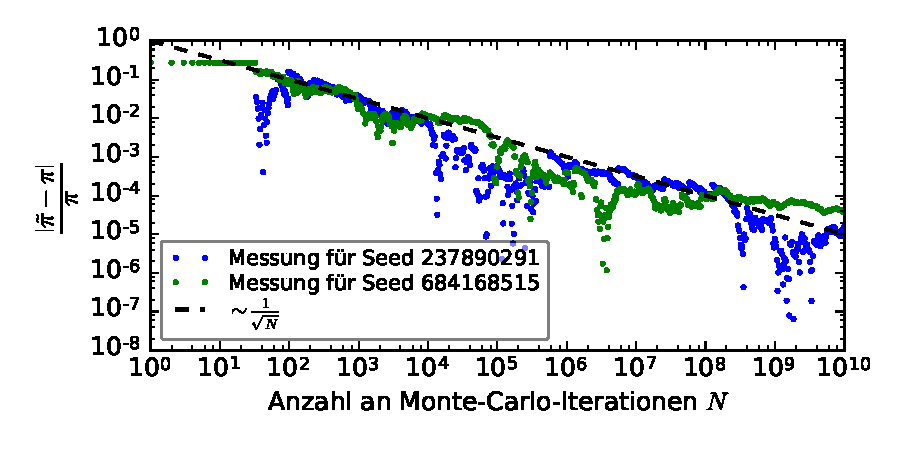
\includegraphics[width=\linewidth]{monte-carlo-pi-error-scaling}
	\end{minipage}
	\caption{captiontext}
	\label{fig:monteerrorfloat}
\end{figure}


\section{Kompilierung}

%Versucht man mit \lstinline!Rootbeer.jar! eine jar-Datei, welche auch Scala-Klassen beinhaltet, in GPU-Code umsetzen zu lassen, z.B. auf diese Weise:
%
%\begin{lstlisting}[language=bash]
%scalac $< -classpath $(ROOTBEER_ROOT)/Rootbeer.jar:. -deprecation
%javac $< -classpath $(ROOTBEER_ROOT)/Rootbeer.jar:.
%scalac $< -classpath $(ROOTBEER_ROOT)/Rootbeer.jar:. -deprecation
%jar -cvfm MontePiGPU.jar.tmp.jar manifest.txt *.class
%java -jar Rootbeer.jar MontePiGPU.jar.tmp.jar MontePiGPU.jar -64bit -computecapability=sm_30
%\end{lstlisting}
%
%Dann kommt es bei soot zu einer Runtime Exception:
%
%\begin{lstlisting}
%java.lang.RuntimeException: cannot get resident body for phantom class : <MonteCarloPiKernel$$anonfun$gpuMethod$1: void <init>(MonteCarloPiKernel,scala.runtime.ObjectRef)>; maybe you want to call c.setApplicationClass() on this class!
%	at soot.SootMethod.retrieveActiveBody(SootMethod.java:316)
%	at soot.rbclassload.RootbeerClassLoader.loadScene(RootbeerClassLoader.java:857)
%	at soot.rbclassload.RootbeerClassLoader.loadNecessaryClasses(RootbeerClassLoader.java:320)
%	at org.trifort.rootbeer.entry.RootbeerCompiler.setupSoot(RootbeerCompiler.java:198)
%	at org.trifort.rootbeer.entry.RootbeerCompiler.compile(RootbeerCompiler.java:219)
%	at org.trifort.rootbeer.entry.RootbeerCompiler.compile(RootbeerCompiler.java:213)
%	at org.trifort.rootbeer.entry.Main.run(Main.java:208)
%	at org.trifort.rootbeer.entry.Main.main(Main.java:244)
%\end{lstlisting}
%
%"Phantom classes are implicitly created models of classes that do not exist on Soot's classpath. To get rid of this problem, make sure that the class you are referencing is on Soot's classpath." \url{http://stackoverflow.com/questions/27383832/why-is-soot-always-saying-that-the-class-i-want-to-load-is-a-phantom-class-even}
%
%Nachdem nun also \lstinline!spark-library.jar! hinzugefügt wurde, verschwindet diese exception, aber Rootbeer findet die Kernel-Implementierung nicht:
%\begin{lstlisting}
%There are no kernel classes. Please implement the following interface to use rootbeer:
%org.trifort.runtime.Kernel
%\end{lstlisting}
%
%Dies könnte daran liegen, das \lstinline!MonteCarloPiKernel.scala! scala benutzt. Dadurch wird für \texttt{soot} verschleiert, dass die Klasse \texttt{Kernel} implementiert.
%Eine Implementierung in java löst das Problem jedoch nicht. Vermutlich weil \texttt{soot} oder \texttt{Rootbeer} nur Klassen analysieren die von der main-Klasse aufgerufen werden. Da die  main-Klasse aber in scala geschrieben ist, ist der Aufruf womöglich für \texttt{soot} nicht sichtbar, sodass \texttt{soot} \texttt{MonteCarloPiKernel.class} als unbenutzt einstuft und ignoriert. Ein Hinweis darauf liefert diese Ausgabe von Soot bei der Ausführung von Rootbeer:
%\begin{lstlisting}
%Total loaded classes: 557
%Total loaded methods: 0
%\end{lstlisting}
%Bei der Java-Version funktioniert die Kompilierung mit Rootbeer und die Ausgabe ist:
%\begin{lstlisting}
%Total loaded classes: 1428
%Total loaded methods: 4385
%\end{lstlisting}
%Eine mögliche Lösung wäre es eine Dummy-Java-Klasse zu schreiben die alle Kernel-Implementierungen aufruft und als main-class im Manifest festgelegt ist.
%Das Problem hierbei ist jedoch, dass Rootbeer Serialisierungs- und Deserialisierungscode in die aufrufende Klasse injeziert. Damit dieser injezierte Code also nicht in die Dummy-Klasse eingesetzt wird, braucht es noch eine Wrapper-Klasse, welche die Kernel-Implementierung aufruft und von der Dummy-Klasse aufgerufen wird. Dies ist \texttt{MonteCarloPi.java}.
%
%Nachdem die Kompilierung mit \texttt{Rootbeer} dann erfolgt ist, muss die Manifest-Datei \texttt{META-INF/MANIFEST.MF} dann nur noch abgeändert werden, damit sie nicht mehr auf die Dummy-Klasse verweist. Durchgeführt wurde es ähnlich, jedoch wurden alle nicht für Rootbeer relevanten Klassen erst nach dem Rootbeer-Aufruf zusammen mit der neuen Manifest-Datei in eine jar-Datei zusammengeführt, siehe Abb.\ref{fig:compilation}.


\begin{figure}[H]
	\centering
	\begin{minipage}{\linewidth}
		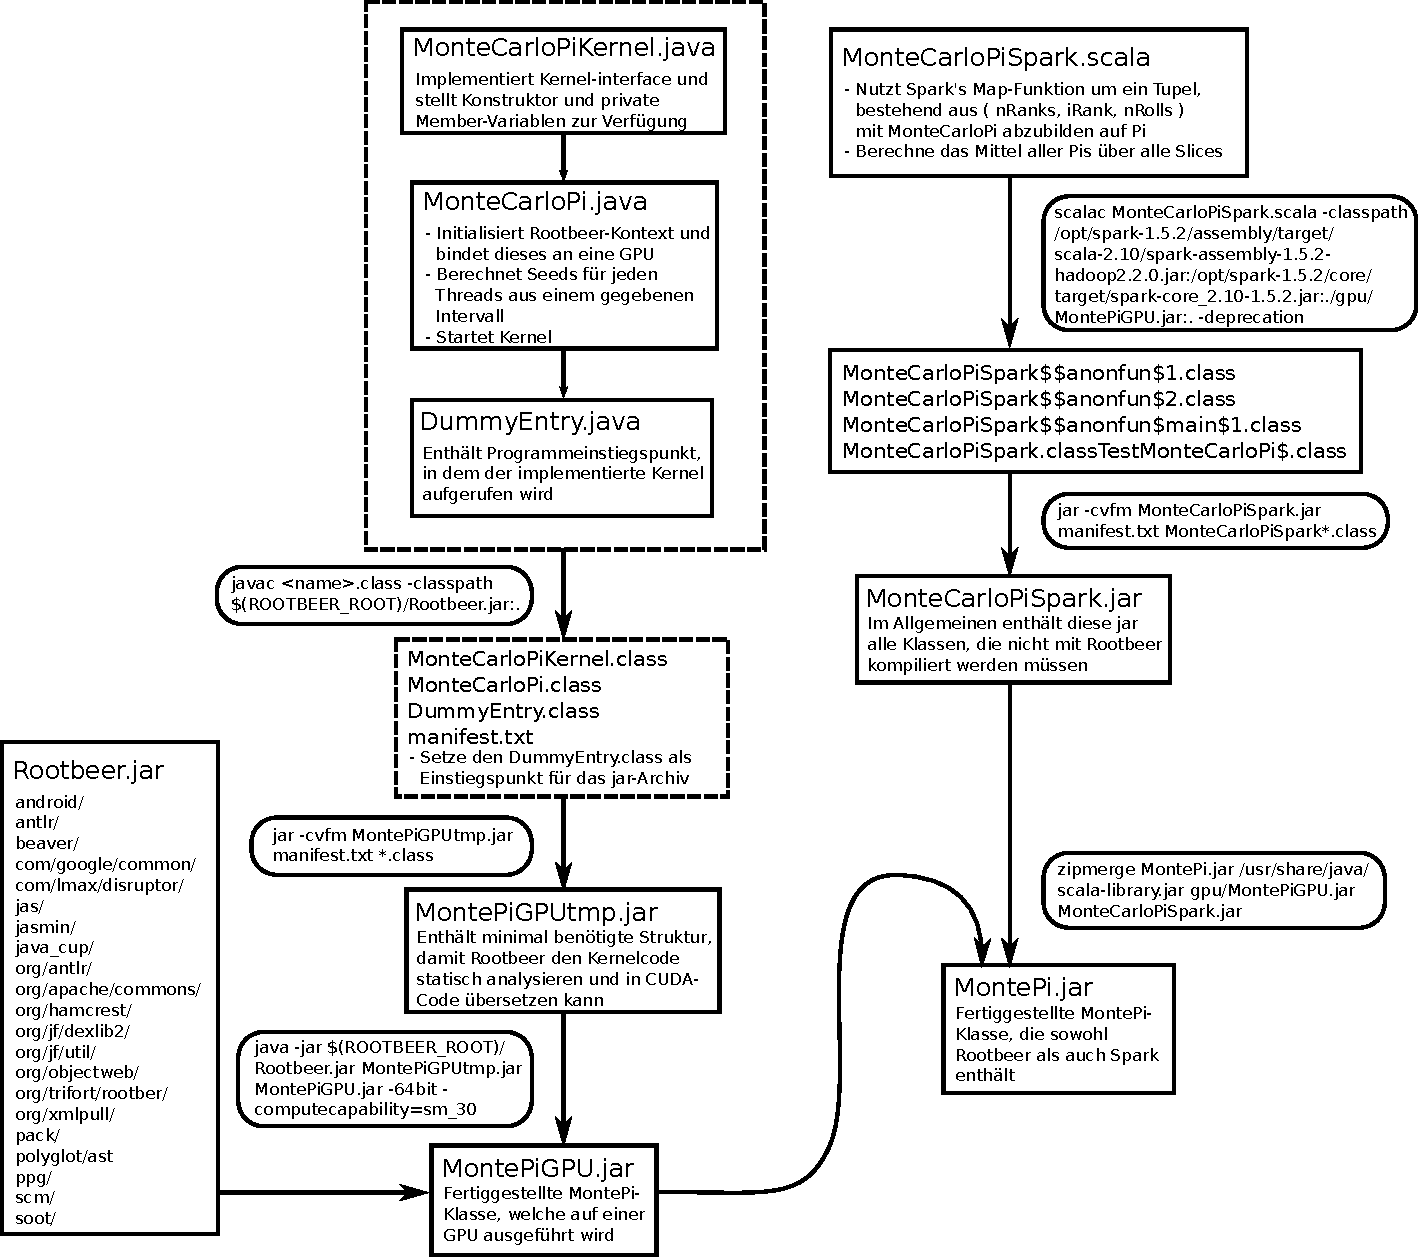
\includegraphics[width=\linewidth]{compile-structure-deu.pdf}
	\end{minipage}
	\caption{Kompilationsschema mit Kommadozeilenbefehlen und Zwischenstati.}
	\label{fig:compilation}
\end{figure}

!!! Problem: Hab mehrere Fehler gefunden deren Kenntnis möglicherweise eine Vereinfachung des Schemas bedeutet. Da bin ich noch am rumspielen, daher ist das halbfertig.

\section{Probleme}
Implementierung:
    Was ist bei GPUs zu beachten ( Seeds, 64-Bit )
    Was ist bei Rootbeer zu beachten?
      - private Variablen werden wirklich immer per memcpy hin und her transportiert.
      - muss nicht auf ungerade Kernel-Zahl achten, werden automatisch aussortiert

%%%%%%%%%%%%%%%%%%%%%%%%%%%%%%%%%%%%%%%%%%%%%%%%%%%%%%%%%%%%%%%%%%%%%%%%%%%%%%%%
\chapter{Leistungsanalyse}
\label{sct:benchmarks}
%%%%%%%%%%%%%%%%%%%%%%%%%%%%%%%%%%%%%%%%%%%%%%%%%%%%%%%%%%%%%%%%%%%%%%%%%%%%%%%%

%%%%%%%%%%%%%%%%%%%%%%%%%%%%%%%%%%%%%%%%%%%%%%%%%%%%%%%%%%%%%%%%%%%%%%%%%%%%%%%%
\section{Testsystem}
\label{sct:taurus}
%%%%%%%%%%%%%%%%%%%%%%%%%%%%%%%%%%%%%%%%%%%%%%%%%%%%%%%%%%%%%%%%%%%%%%%%%%%%%%%%


Für die Skalierungstests wurde Taurus, einer der Hochleistungsrechner der TU-Dresden, benutzt.
Der Bau der ersten Phase von Taurus war 2013 abgeschlossen\cite{taurusnutzerschulung}.
Zum Zeitpunkt der Nutzung (2015/2016) waren alle Knoten von Phase 1, vgl. \autoref{fig:taurusphase1} links, in die 2015 fertiggestellt\cite{heisehrsk2} Phase 2, siehe \autoref{fig:taurusphase1} rechts, integriert \cite{doctudtaurushardware}. Gerechnet wurde je nach Verfügbarkeit auf Phase 1 oder 2 von Taurus, vgl. Tabelle~\ref{tbl:island2}.

\begin{figure}[H]
	\centering
	\begin{minipage}{0.5\linewidth}
		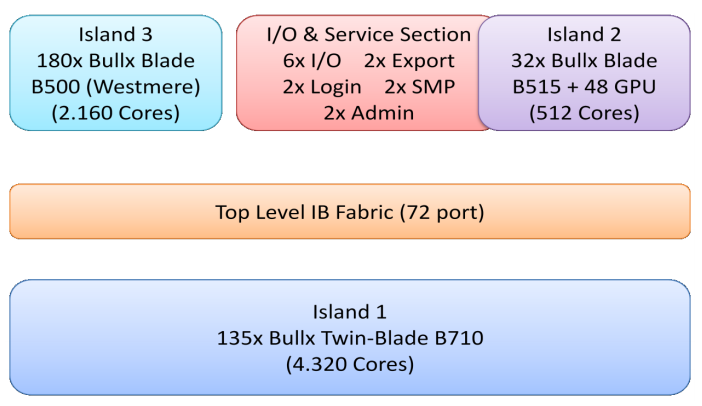
\includegraphics[width=\linewidth]{taurusphase1}
	\end{minipage}\begin{minipage}{0.5\linewidth}
		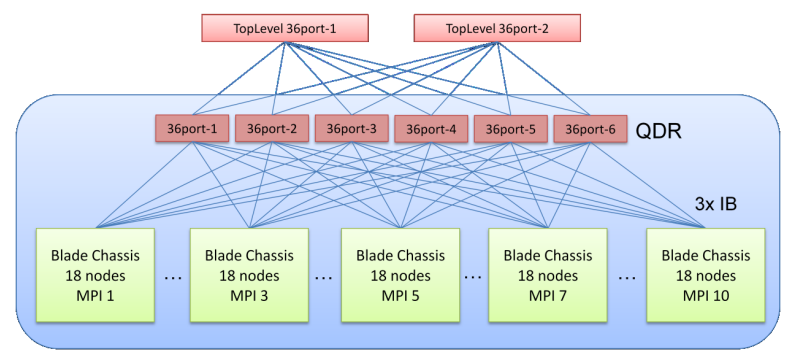
\includegraphics[width=\linewidth]{taurusphase1island1interconnects}
	\end{minipage}
	\caption{\textbf{Links:} Übersicht Taurus Phase 1. \textbf{Rechts:} Schema der Topologie von Insel 2, auf der ausschließlich gerechnet wurde. Die Bilder wurden übernommen aus Ref.\cite{taurusnutzerschulung}}
	\label{fig:taurusphase1}
\end{figure}

\begin{table}[H]
	\begin{tabularx}{0.9\linewidth}{r|Y|Y}
		& \textbf{Phase 1} & \textbf{Phase 2} \\
		\hline
		Knoten          & 44 & 64 \\
		Hostnamen       & taurusi2[001-044] & taurusi2[045-108] \\
		Prozessor       & 2x Intel Xeon CPU E5-2450 (8 Kerne) zu je \SI{2.10}{\giga\hertz}, MultiThreading deaktiviert, AVX, 2x 268.8\,GSPFLOPS \cite{2400flops}
						& 2x Intel(R) Xeon(R) CPU E5-2680 v3 (12 Kerne) zu je \SI{2.50}{\giga\hertz}, MultiThreading deaktiviert, AVX2 insbesondere FMA3\cite{ark2680v3}, 2x 480\,GSPFLOPS\cite{e5microway} \\
		GPU 			& 2x NVIDIA Tesla K20X & 4x NVIDIA Tesla K80 \\
		Arbeitsspeicher & \SI{32}{\gibi\byte} & \SI{64}{\gibi\byte} \\
		Festplatte      & \SI{128}{\gibi\byte} SSD & \SI{128}{\gibi\byte} SSD
	\end{tabularx}
	\caption{Zusammensetzung Insel 2 von Taurus\cite{doctudtaurussystem}}
	\label{tbl:island2}
\end{table}

\begin{table}[H]
	\begin{tabular}{r|c|c}
	& \textbf{K20X} & \textbf{K80} \\
	\hline
	Chip       & GK110 & GK210 \\
	Takt       & \SI{0.732}{\giga\hertz} & \SI{0.560}{\giga\hertz} \\
	CUDA-Kerne & 2688 & 4992 \\
	Speicher   & \SI{6}{\gibi\byte}, GDDR5 384 Bit Busbreite
	           & $2\times\SI{12}{\gibi\byte}$, GDDR5 384 Bit Busbreite \\
    Bandbreite & \SI{250}{\giga\byte\per\second}
	           & $2\times\SI{240}{\giga\byte\per\second}$              \\
%	\begin{minipage}{2.5cm}\begin{flushright}Theoretische\\Spitzenleistung\end{flushright}\end{minipage} & 3935\,GSPFLOPS, 1312\,GDPFLOPS
%					& 5591\,GSPFLOPS, 1864\,GDPFLOPS \\
	Theoretische    & 3935\,GSPFLOPS & 5591\,GSPFLOPS \\
	Spitzenleistung & 1312\,GDPFLOPS & 1864\,GDPFLOPS
	\end{tabular}
	\caption{Spezifikationen der Kepler-Grafikkarten von Taurus\cite{nvidiakepler,k20anandtech}}
	\label{tbl:k20k80}
\end{table}

Zu den Spitzenleistungen in Tabelle~\ref{tbl:k20k80} sei angemerkt, dass jeder CUDA-Kern eine Operation einfacher Fließkommagenaugigkeit oder eine 32-Bit Integeroperation berechnen kann und dass auf drei CUDA-Kerne eine Doppelpräzisionseinheit kommt, wodurch sich die DFLOPS berechnen.
Die K80 hat außerdem einen Boost-Modus mit \SI{0.875}{\giga\hertz}, also einer Leistungssteigerung von $1.56$.

Für z.B. die Tesla K20X beträgt die Maximalleistung in der Berechnung von Fließkommazahlen einfacher Genauigkeit (Single Precision Floating Point Operations Per Second - SPFLOPS) im Verhältnis einer Multiplikation zu einer Addition:
\begin{align}
	\SI{0.732}{\giga\hertz} \cdot 2688\,\text{CUDA-Kerne} \cdot
	1\,\frac{ \text{FMA-Einheit} }{ \text{CUDA-Kern} } \cdot
	2\,\frac{ \text{SPFLO} }{ \text{FMA-Einheit} }
	= 3935\,\text{GSPFLOPS}
\end{align}

Für den z.B. den Xeon E5-2680 v3 Prozessor beträgt die Maximalleistung:
\begin{align}
	\SI{2.50}{\giga\hertz} \cdot
	12\,\text{Kerne} \left(
		1\,\frac{ \text{AVX ADD Einheit} }{ \text{Kern} } +
		1\,\frac{ \text{AVX MUL Einheit} }{ \text{Kern} }
	\right) \cdot
	8\,\frac{ \text{SPFLO} }{ \text{AVX Einheit} } \\
	= 480\,\text{GSPFLOPS}
\end{align}


%%%%%%%%%%%%%%%%%%%%%%%%%%%%%%%%%%%%%%%%%%%%%%%%%%%%%%%%%%%%%%%%%%%%%%%%%%%%%%%%
\section{Profiling}
%%%%%%%%%%%%%%%%%%%%%%%%%%%%%%%%%%%%%%%%%%%%%%%%%%%%%%%%%%%%%%%%%%%%%%%%%%%%%%%%

Profiling mit dem NVIDIA Visual Profiler ist auch mit Rootbeer möglich.
Dafür muss als ausführbare zu analysierende Datei jedoch \lstinline!java! mit den Argumenten zu der auszuführenden JAR-Datei angegeben werden:
\begin{lstlisting}[language=bash, caption={Erstellen der Profiling-Daten}, label={lst:nvprof}]
sbatch --time=00:30:00 --nodes=1 --partition=gpu2 --cpus-per-task=4 --gres='gpu:4' <<EOF
#!/bin/bash
nvprof --analysis-metrics --metrics all \
-o $HOME/scaromare/MontePi/profilingDataMultiGpuScala.nvp%p \
$(which java) -jar $HOME/scaromare/MontePi/singleNode/multiGpu/scala/MontePi.jar $((2*14351234510)) 2
EOF
\end{lstlisting}
Die so erzeugten Zeitmessungen in \lstinline!profilingDataMultiGpuScala.nvp! können mit \lstinline!nvvp! ausgewertet und visualisiert werden.

In \autoref{fig:apicalls} ist ein Programmlauf mit zwei Grafikkarten zu sehen.
In der originalen Rootbeerversion wurde für jede Grafikkarte erst ein \lstinline!cuCtxCreate! aufgerufen, welches sehr zeitaufwändig ist, dann der freie Grafikkartenspeicher der Grafikkarte abgerufen und zuletzt der Kontext wieder mit \lstinline!cuCtxDestroy! gelöscht, siehe auch Seite~\pageref{pg:cuCtxCreate} und \autoref{fig:apicalls} oben.
Dies wurde im eigenen Fork behoben, sodass nur noch ein Aufruf zu \lstinline!cuCtxCreate! für die Grafikkarte, die auch wirklich benutzt wird, notwendig ist, siehe \autoref{fig:apicalls} unten.
Die Gesamtlaufzeit im Beispiel wurde so von ca. \SI{8}{\second} auf \SI{5}{\second} reduziert.

\begin{figure}
	\begin{center}
		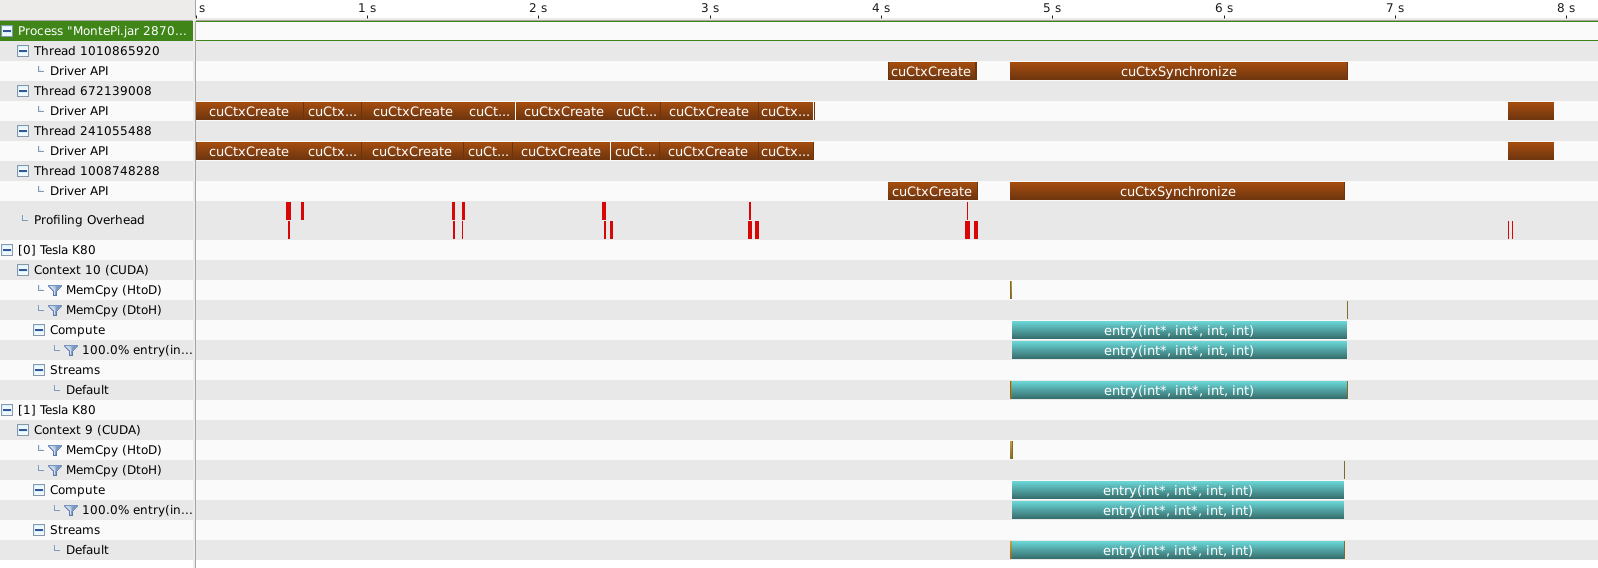
\includegraphics[width=\linewidth]{../MontePi/profiling/2of4-APICalls.png}\\
		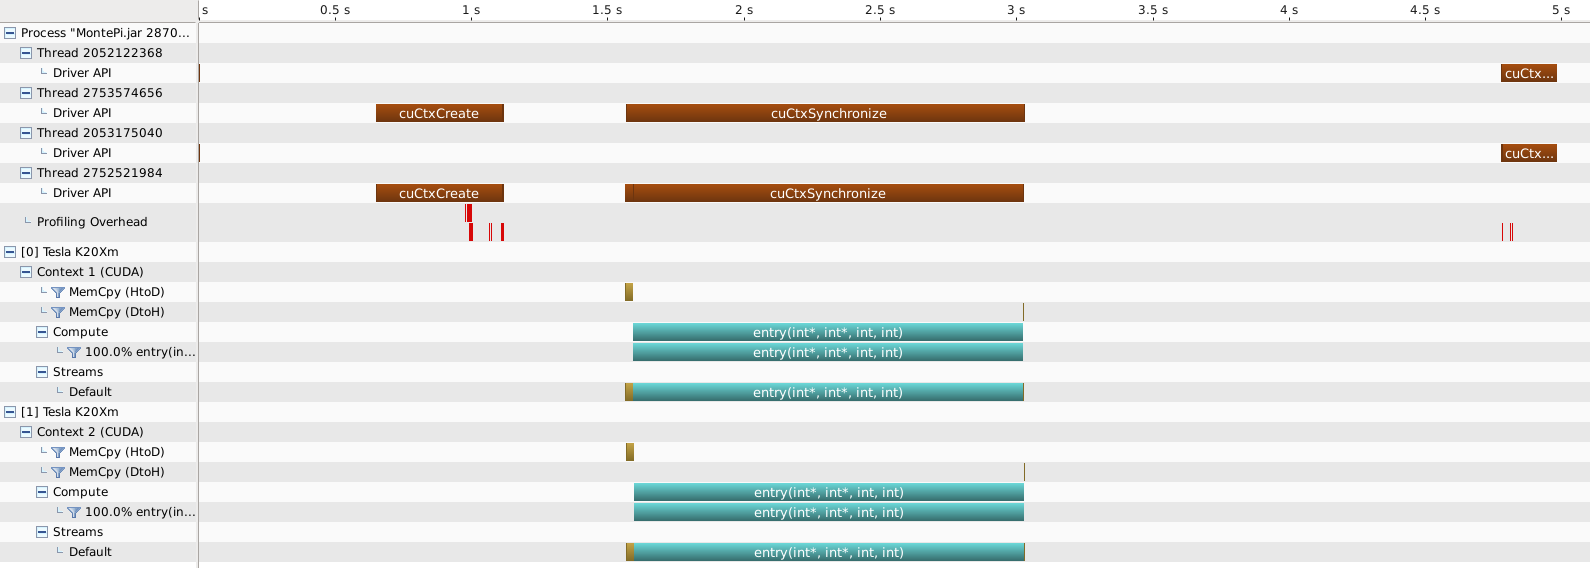
\includegraphics[width=\linewidth]{../MontePi/profiling/2of2-afterLoadDevicesPerformanceFix.png}
	\end{center}
	\caption{Profiling der CUDA-API-Aufrufe. \textbf{Oben:} Vor dem \lstinline!cuCtxCreate!-Fix im Rootbeerfork ausgeführt auf einem Tesla K80-Knoten. \textbf{Unten:} Nach dem Fix ausgeführt auf einem Tesla K20X-Knoten.}
	\label{fig:apicalls}
\end{figure}


%%%%%%%%%%%%%%%%%%%%%%%%%%%%%%%%%%%%%%%%%%%%%%%%%%%%%%%%%%%%%%%%%%%%%%%%%%%%%%%%
\section{Monte-Carlo-Simulation verschiedener Implementationen}
%%%%%%%%%%%%%%%%%%%%%%%%%%%%%%%%%%%%%%%%%%%%%%%%%%%%%%%%%%%%%%%%%%%%%%%%%%%%%%%%

In Abb.\ref{fig:montepiworkloadscaling} wurde die Ausführungszeit von Monte-Carlo-Simulationen implementiert mit verschiedenen Programmiersprachen über die Anzahl an Monte-Carlo-Iterationen gemessen.
Die Zeit wurde mit dem Linux \lstinline!time!-Befehl gemessen. Dieser Befehl gibt real-, user- und sys-Zeit aus; die real-Zeit wird für den Benchmark genutzt.

Jede Implementation hat eine gewisse Initialisierungszeit. Bei der C++-Version beträgt diese jedoch nur knapp \SI{70}{\milli\second}, während die reine Java-Version schon ca. \SI{220}{\milli\second} benötigt.
Die Nutzung von Scala erhöht dies auf \SI{250}{\milli\second} und die Nutzung von Rootbeer führt eine weitere Initialisierungszeit von \SI{2}{\second} ein, sodass für wenig Iterationen die Rootbeerversion bis zu 20x langsamer sind als die Hostprozessorversionen.
Die Rootbeerinitialisierungszeit beinhaltet das Entpacken der benötigten Binärdateien, das Erstellen des CUDA-Kontextes und den Transfer der Daten zwischen GPU und Host.
Die hier nicht gemessene Spark-Implementierung benötigte in Einzeltests noch mehr Zeit für die Initialisierung.

Erst für 10 Milliarden Iterationen beginnt die Initialisierungszeit der Rootbeer-Implementierungen im Vergleich zur Rechenzeit vernachlässigbar zu werden, sodass ab da die Lastenskalierung ein lineares Verhalten annimmt.
Bei der C++-Version ist dies indes schon bei ca. 100 Millionen Iterationen der Fall.
\begin{figure}
	\centering
	\begin{minipage}{0.7\linewidth}
		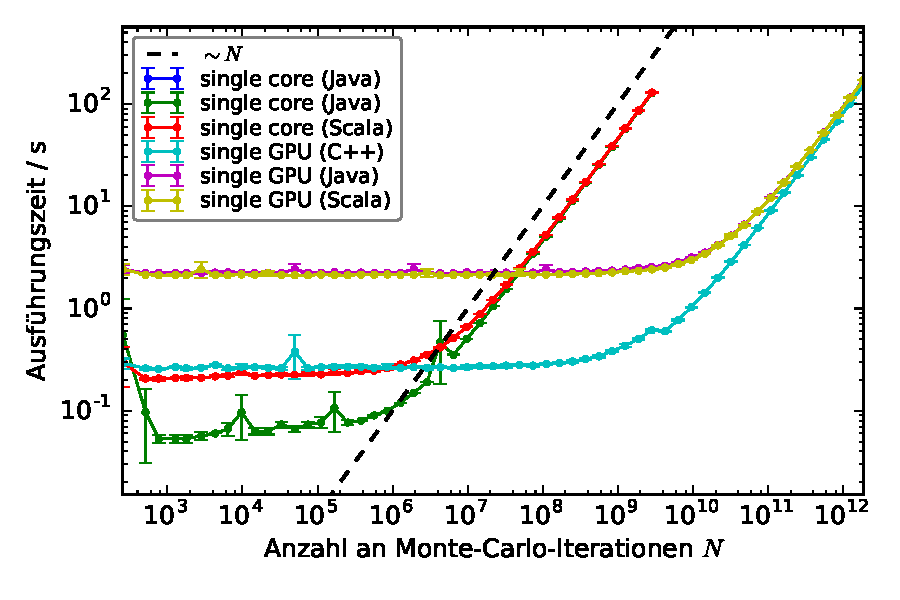
\includegraphics[width=\linewidth]{../MontePi/benchmark/benchmarks-workload-scaling.pdf}
	\end{minipage}
	\caption{Benötigte Ausführungszeit der Monte-Carlo Pi-Berechnung in Abhängigkeit von der Anzahl an Iterationen. Getestet auf Taurusknoten \lstinline!taurusi2095! und \lstinline!taurusi2105!, also auf Tesla K80-Knoten, siehe \autoref{sct:taurus}}
	\label{fig:montepiworkloadscaling}
\end{figure}

Weiterhin ist aus dem Plot abzulesen, dass für große Lasten wie z.B. für drei Milliarden Iterationen die Versionen, die von Grafikarten Gebrauch machen, um einen Faktor $50$ (Scala) bis $210$ (C++) schneller sind als die Implementierungen, die auf einem Prozessor-Kern ausgeführt werden.
Die theoretische Maximalleistung eines Kerns auf dem Intel Xeon E5-2680v3-Knoten beträgt $40\,\text{GSPFLOPS}$.
Das heißt man würde einen Speedup von ca. $140\,\text{GSPFLOPS}$ erwarten.
Dass der Speedup höher ist liegt wahrscheinlich daran, dass Java keinen oder nur schlecht optimierten Gebrauch von AVX für die Monte-Carlo-Berechnung macht.

\begin{figure}[H]
	\centering
	\begin{minipage}{0.7\linewidth}
		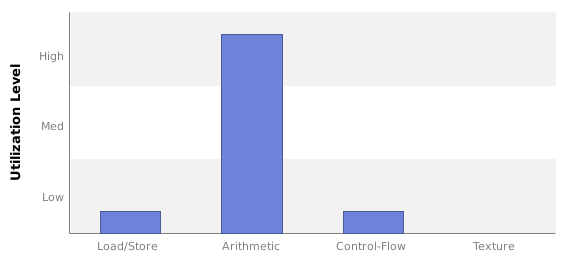
\includegraphics[width=\linewidth]{../presentation/kernel-utilization}
	\end{minipage}
	\caption{Auswertung der Kernel-Utilisierung mit dem NVIDIA Visual Profiler des mit Rootbeer beschleunigten Monte-Carlo-Algorithmus.}
	\label{fig:utilization}
\end{figure}


Die Auswertung der Utilisierung in \autoref{fig:utilization} zeigt, dass der Algorithmus die arithmetischen Einheiten fast voll auslastet.
Es ist also noch Spielraum für Algorithmen die weniger rechenlastig sind und mehr Speicherzugriffe haben.
Im Allgemeinen wird es sich aber nicht lohnen Algorithmen zu parallelisieren, die gleich viel Speicherzugriffe wie Berechnungen haben.
Gut geeignet sind Algorithmen, bei denen die Anzahl an Berechnungen mit dem Quadrat der Anzahl an Speicherzugriffen oder noch schneller steigt.


%%%%%%%%%%%%%%%%%%%%%%%%%%%%%%%%%%%%%%%%%%%%%%%%%%%%%%%%%%%%%%%%%%%%%%%%%%%%%%%%
\section{Monte-Carlo-Simulation mit Spark und Rootbeer}
%%%%%%%%%%%%%%%%%%%%%%%%%%%%%%%%%%%%%%%%%%%%%%%%%%%%%%%%%%%%%%%%%%%%%%%%%%%%%%%%

In Abbildung~\ref{fig:montepiweakscaling} ist die Laufzeit über die Anzahl an Grafikkarten dargestellt. jeder Knoten hat zwei Tesla K20X-Grafikkarten.
Die Anzahl an Iterationen wurde proportional zu der Anzahl an Grafikkarten erhöht, sodass jede Grafikkarte immer gleich viel Arbeit hat.
Man erwartet also, dass die Ausführungszeit unabhängig von der Anzahl an Grafikkarten konstant bleibt, wie es auch der Fall ist.

Ab 16,17,18, in einem Einzelfall auch 19 Grafikkarten steigen jedoch die Laufzeiten plötzlich um ca. \SI{1}{\second} an, sodass der Speedup sich vom idealen Speedup entfernt, das heißt die parallele Effizienz nimmt ab.
Die genaue Ursache hierfür wurde nicht gefunden.
Mögliche Ursachen könnte Spark, Straggler, das Verbindungsnetzwerk oder vielleicht auch Rootbeer sein.
Interessant wäre auch eine Wiederholung des Tests auf einem K80-System und jeweils mit mehr als 32 Grafikkarten, um eine weitere Erhöhung der Laufzeit bei Vielfachen von 16 Grafikkarten auszuschließen.
Aus Rechenzeitgründen war dies jedoch zum aktuellen Zeitpunkt nicht mehr möglich.

\begin{figure}[H]
	\centering
	\begin{minipage}{0.5\linewidth}
		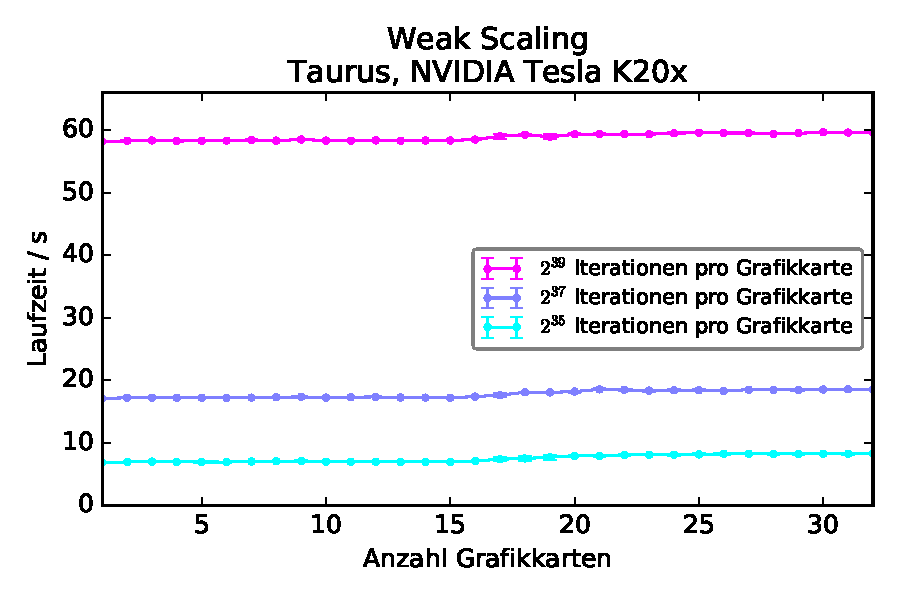
\includegraphics[width=\linewidth]{../MontePi/benchmark/weak-scaling-time-gpu.pdf}
	\end{minipage}\begin{minipage}{0.5\linewidth}
		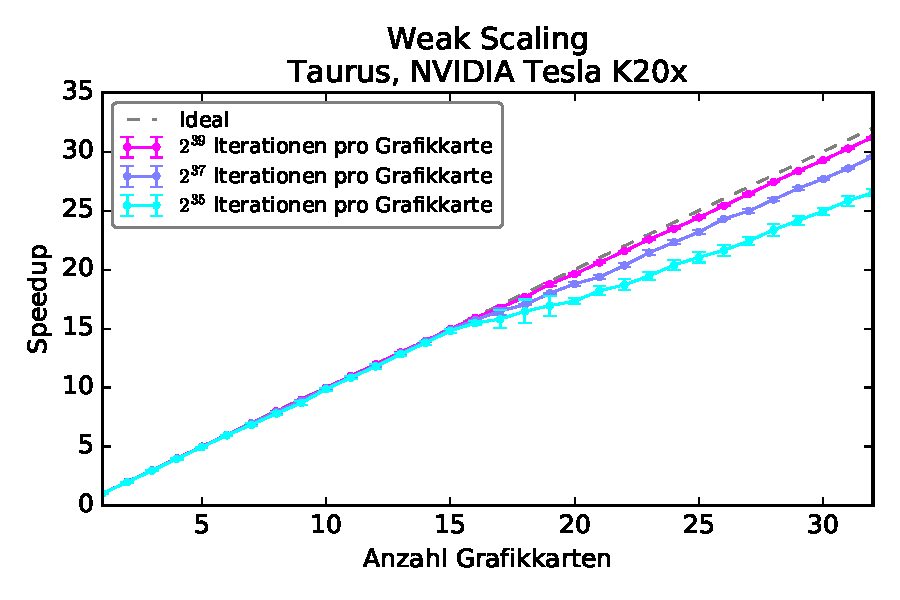
\includegraphics[width=\linewidth]{../MontePi/benchmark/weak-scaling-speedup-gpu.pdf}
	\end{minipage}
    \centerline{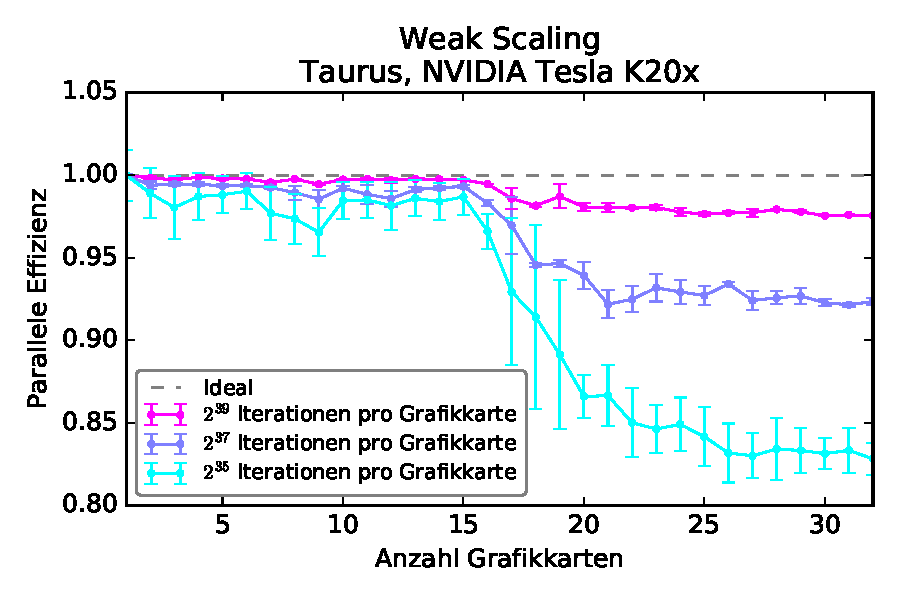
\includegraphics[width=0.5\linewidth]{../MontePi/benchmark/weak-scaling-efficiency-gpu.pdf}}
	\caption{Benötigte Ausführungszeit der Monte-Carlo Pi-Berechnung in Abhängigkeit von der Anzahl an Grafikkarten gemessen auf Tesla K20X-Knoten. \textbf{Links:} Absolute Ausführungszeiten der Spark-Map-Funktion. \textbf{Rechts:} Speedup bezüglich der Laufzeit mit einer Grafikkarte. \textbf{Unten:} Parallele Effizienz}
	\label{fig:montepiweakscaling}
\end{figure}

Weiterhin wurden die Benchmarks wiederholt für vier fixierte Totalproblemgrößen, sodass die Arbeit pro Grafikkarte mit Erhöhung der Parallelisierung abnimmt.
Wie man in \autoref{fig:montepistrongscaling} sieht nimmt also mit Erhöhung der Grafikkarten die Laufzeit so lange proportional ab, bis der Großteil der benötigten Zeit nur noch aus der seriellen Initialisierungszeit besteht und sich somit der wirklich erreichte Speedup sättigt, vergleiche auch mit dem Amdahlschen Gesetz.

Für $2^37=137\cdot 10^9$ Gesamtiterationen ist der Speedup bei ungefähr vier gesättigt.
Es ist also nicht sinnvoll dieses dieses Problem mit signifikant mehr als vier Grafikkarten zu parallelisieren.
Wie aus \autoref{fig:montepiworkloadscaling} entnehmbar würde die CPU-Version ungefähr \SI{500}{\second} benötigen.
Es ist also erst bei sehr großen Problemen, die auf dem Host mehr als eine Minute benötigen würden, überhaupt sinnvoll Grafikkarten einzusetzen.

Wenn auf dem Host AVX und alle Kerne benutzt werden, dann muss das Problem noch größer sein, damit sich Grafikkarten lohnen.
Wenn die Probleme aber genügend groß sind, dann rentieren sich Grafikkartenbeschleuniger sehr.
Bei ungefähr vergleichbaren Prozessoren zu Grafikkarten und beiderseits sehr gut optimierten Programmen ist, wie in \autoref{tbl:k20k80} an den theoretischen Peak-FLOPS zu sehen, ein 10-facher Geschwindigkeitsgewinn realistisch.
Dies gilt jedoch nur für einfache Genauigkeit.
Für Fließkommaberechnungen doppelter Genauigkeit sind Grafikkarten je nach Modell ungeeignet.

\begin{figure}[H]
	\centering
	\begin{minipage}{0.5\linewidth}
		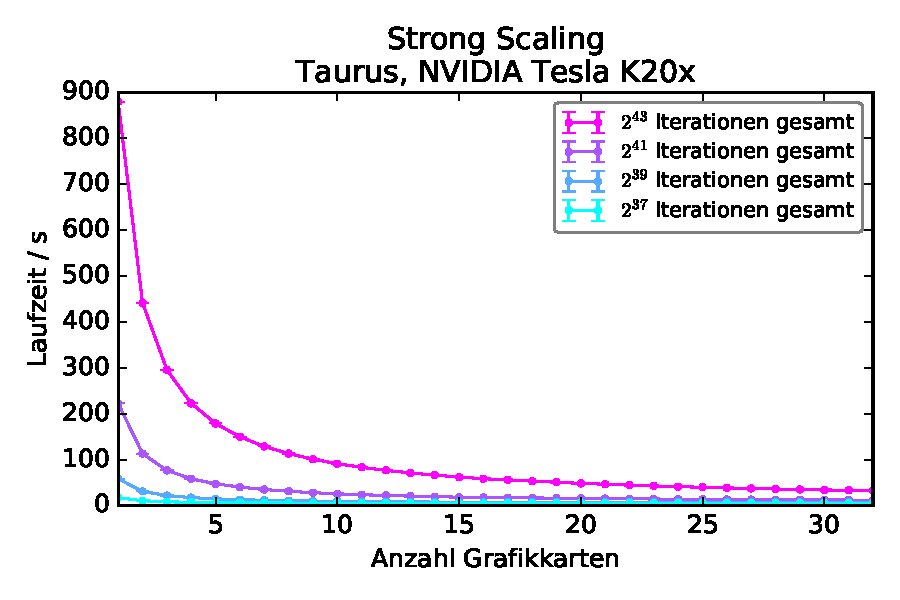
\includegraphics[width=\linewidth]{../MontePi/benchmark/strong-scaling-time-gpu.pdf}
	\end{minipage}\begin{minipage}{0.5\linewidth}
		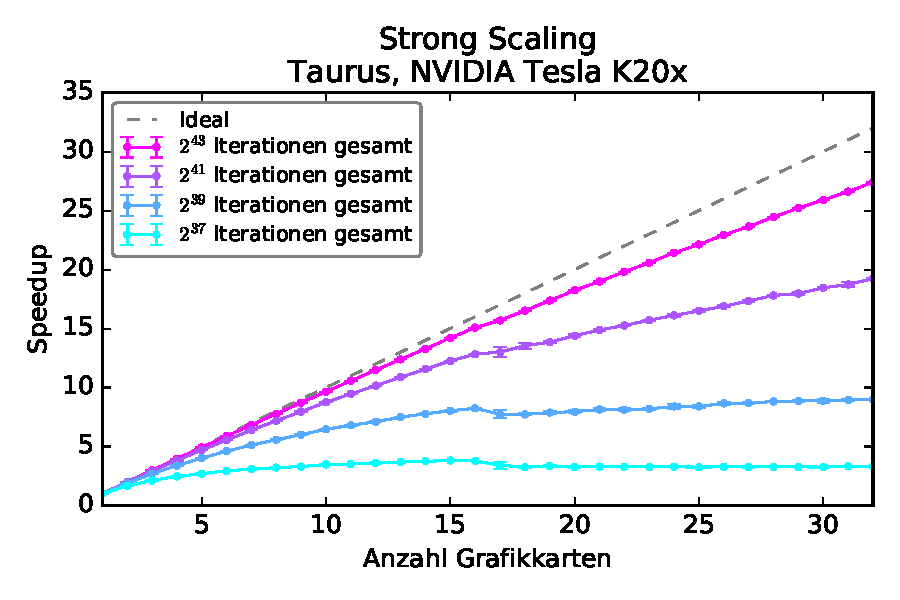
\includegraphics[width=\linewidth]{../MontePi/benchmark/strong-scaling-speedup-gpu.pdf}
	\end{minipage}
    \centerline{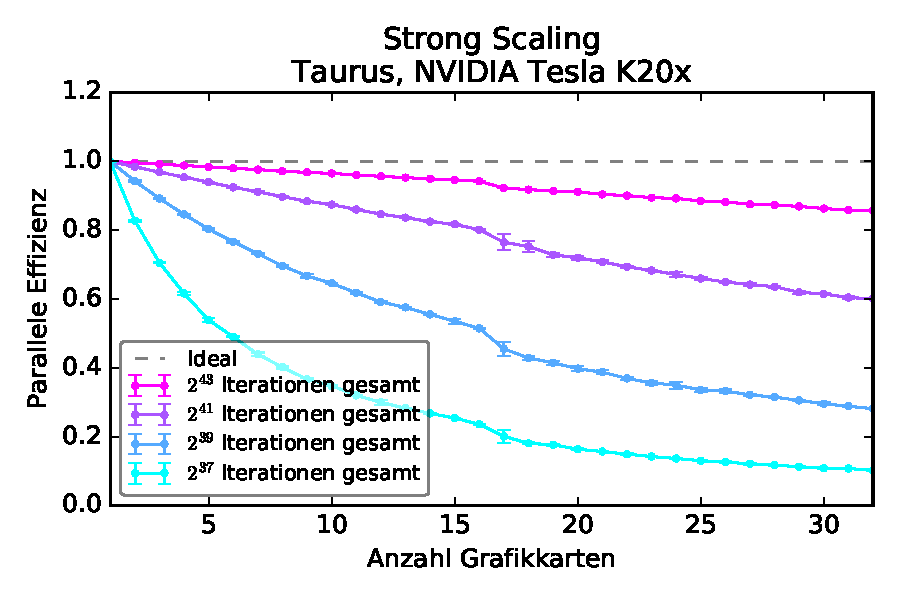
\includegraphics[width=0.5\linewidth]{../MontePi/benchmark/strong-scaling-efficiency-gpu.pdf}}
	\caption{Benötigte Ausführungszeit der Monte-Carlo Pi-Berechnung in Abhängigkeit von der Anzahl an Grafikkarten gemessen auf Tesla K20X-Knoten. \textbf{Links:} Absolute Ausführungszeiten der Spark-Map-Funktion. \textbf{Rechts:} Speedup bezüglich der Laufzeit mit einer Grafikkarte. \textbf{Unten:} Parallele Effizienz}
	\label{fig:montepistrongscaling}
\end{figure}


\chapter{Zusammenfassung}

% um was gehts (Kontext) -> ist doch schon in der Einleitung :S? Außerdem wird das indirekt bei dem nächsten Punkt erwähnt

% Was habe ich gemacht
Im Rahmen dieser Belegarbeit wurde erfolgreich ein simpler rechenlastiger Monte-Carlo-Algorithmus mit Spark und Rootbeer auf einem Grafikkartencluster parallelisiert und gebenchmarkt.
Die Benchmarkresultaten zeigen, dass es sich schon lohnen kann Probleme, die mehrere Sekunden auf einem x86-Prozessor benötigen würden, auf Grafikkarten zu parallelisieren.
Die gemessenen Geschwindigkeitsgewinne sind für den Algorithmus vergleichbar mit den theoretischen Speedups, welche sich aus den theoretischen Peak-Flops berechnen.
Dafür war jedoch zeitintensive Einarbeitung in den Rootbeerquellcode nötig, um mehrere Bugs zu lösen.
Ein angepasster Fork von Rootbeer befindet sich in \cite{ownrootbeerfork} und die Beispielquellcodes zu Spark in Verbindung mit Rootbeer befinden sich in \cite{scaromare}.\\

% Was haben wir gelernt -> schon mit in obigem Absatz mehr oder minder enthalten

% Ausblick

Ausgehend von dieser Arbeit wäre es interessant einen komplexeren Algorithmus mit mehr Speicherzugriffen und mehr Kommunikation innerhalb von Spark zu testen.
Falls zwischen iterativen Rootbeerkernelaufrufen Daten auf der Grafikkarte wiederbenutzt werden können, dann wäre es sinnvoll Rootbeer so zu erweitern, dass man Speicher in der Grafikkarte behalten und für den nächsten Kernelaufruf wiederverwenden kann.
Eine interessante Anwendung wäre z.B. das maschinelle Lernen auf einem Grafikkartencluster.

Weiterhin könnte man Straggler besser ausgleichen wenn man wie in Spark gewohnt ungefähr vier mal so viele Partitionen, d.h. Teilaufgaben, schedulen könnte als es Grafikkarten zur Verfügung gibt.
Mit der hier vorliegenden Version ist dies nicht einfach möglich, da die Verteilung der Partitionen an die Grafikkarten statisch vor der Ausführung geschieht.
Das Problem hierbei ist jedoch, dass mit CUDA nicht dynamisch festgestellt werden kann, welche Grafikkarten in Benutzung sind und welche nicht.



%\setlength{\headheight}{27pt} % needed because zih-template is buggy as *** and the chapter title is too long for the standard header
%\setlength{\headheight}{17pt}

\appendix

\chapter{Standardabweichung des Mittelwertes}
\label{apx:meanerror}

Dieses Kapitel richtet sich leicht nach Ref.\cite{meanerrorulm}. Sei $f\equiv(f_i)$ eine Folge von $N$ Stichproben aus einer Zufallsverteilung mit einem Mittelwert $\mu$ und $\mu_N$ der empirische Mittelwert dieser Folge. Die Differenz $\Delta_N:=\mu-\mu_N$ wird nun abgeschätzt mit der Standardabweichung einer Folge von empirischen Mittelwerten $\left(\mu_{N,k}\right)$ die alle mit (sehr wahrscheinlich) verschiedenen Folgen bzw. Vektoren $(f_i)$ gebildet seien.

Sei nun $\langle \cdot \rangle_N: \mathbb{S}\times \mathbb{R}^N \rightarrow \mathbb{R}^N, \langle (f_i)_k \rangle_N:= \frac{1}{N}\sum\limits_{i=0}^N {f_i}_k$ der empirische Mittelwert und $E(\cdot):\mathbb{S}\rightarrow \mathbb{R}, E\left( x_k \right):= \lim\limits_{N\rightarrow \infty} \frac{1}{N} \sum\limits_{k=0}^N f_k$ der Erwartungswert über eine unendlich Folge aus einem beliebigen statistischen Werten für begrenzte Folgen $(f_i)$. Hierbei ist $\mathbb{S}$ der Raum der Folgen. Aus der Definition der beiden Mittelwerte wird klar, dass man die Summen und damit die Bildung der Mittelwerte vertauschen kann, sofern ein Grenzwert existiert. Dies wird in Gleichung~\ref{eq:EabToEaEb-pre} angewandt.
%\\  = \frac{1}{N} E\left( \sigma_k \right)
%    + E\left( \left( \mu_{N,k}-\mu \right)
%      \frac{1}{N} \sum\limits_{j=0,j\neq i}^N \left( f_{jk}-\mu \right) \right)
%\\  \approx \frac{1}{N} E\left( \sigma_k \right) +
%      E\left( \frac{1}{N} \sum\limits_{i=0}^N \left( f_{ik}-\mu \right)
%      \left( \mu_{N,k'} - \mu \right) \right) \\
%	= \frac{\sigma}{N} +  E\left( \left(\mu_{N,k} - \mu \right)
%	  \left( \mu_{N,k} - \mu \right) \right)
%   = \frac{\sigma}{N} +  E\left( \mu_{N,k} - \mu \right)
%	  E\left( \mu_{N,k} - \mu  \right) \\
%	= \frac{\sigma}{N} +  \left( \mu - \mu \right)\left( \mu - \mu  \right)
\begin{align}
	\sigma_{\mu_N}^2
   := E\left( \left( \mu_N - \mu \right)^2 \right)
   := E\left( \left( \langle f_{ik} \rangle_N - \mu \right)^2 \right)
	= E\left( \langle f_{ik} - \mu \rangle_N^2 \right)
\\  = E\left(
	  \left( \frac{1}{N} \sum\limits_{i=0}^N \left(f_{ik}-\mu\right) \right)
	  \left( \frac{1}{N} \sum\limits_{i=0}^N \left(f_{ik}-\mu\right) \right)
	  \right)
	= E\left( \frac{1}{N^2} \sum\limits_{i=0}^N \sum\limits_{j=0}^N
		      \left( f_{ik}-\mu \right) \left( f_{jk}-\mu \right) \right)
    \\
	\label{eq:EabToEaEb-pre}
	= \frac{1}{N} E\left(
		 \frac{1}{N} \sum\limits_{i=0}^N \left( f_{ik}-\mu \right)^2
      \right)
    + E\left( \frac{1}{N} \sum\limits_{i=0}^N \left( f_{ik}-\mu \right)
      \frac{1}{N} \sum\limits_{j=0,j\neq i}^N \left( f_{jk}-\mu \right) \right)
    \\
	\label{eq:EabToEaEb-post}
    = \frac{1}{N} E\left( \sigma_k \right)
    + \frac{1}{N} \sum\limits_{i=0}^N
      \frac{1}{N} \sum\limits_{j=0,j\neq i}^N
      \left( \underbrace{E\left(f_{ik}\right)}_{=\mu}-\mu \right)
      \left( \underbrace{E\left(f_{jk}\right)}_{=\mu}-\mu \right)
	= \uuline{ \frac{\sigma}{N} }
\end{align}
Man beachte, dass der Schritt in Gl.\ref{eq:EabToEaEb-pre}-\ref{eq:EabToEaEb-post} nur möglich ist, wenn $f_i$ unabhängig von $f_j$ ist, was hier der Fall ist, da der einzige abhängige Fall für $i=j$ aus der SUmme rausgezogen würde, sodass $E(a b)=E(a)E(b)$ anwendbar ist.

Man beachte, dass der zweite Summand nur durch die Mittelung über mehrere komplett verschiedene Versuchsreihen Null wird. Betrachtet man jedoch nur eine Versuchsreihe, dann hat der zweite Summand auch ein Skalierverhalten in Abhängigkeit zu $N$. Da aber das Vorzeichen wechseln kann, muss man den Betrag betrachten:
\begin{align}
	\frac{1}{N} \sum\limits_{i=0}^N \left( f_i-\mu \right)
    \frac{1}{N} \sum\limits_{j=0,j\neq i}^N \left( f_j-\mu \right)
    =
	\frac{1}{N} \sum\limits_{i=0}^N
    \frac{1}{N} \sum\limits_{j=0,j\neq i}^N
    \left( f_i f_j - \mu \left( f_i + f_j \right) + \mu^2 \right)
    \\
    \label{eq:approxmuN}
    \approx
	\mu_N^2 - 2 \mu \mu_N + \mu^2
	\overset{ \mu_N \approx \mu - \sigma_{\mu_N} }{\approx}
	\mu^2 - 2 \sigma_{\mu_N} \mu + \sigma_{\mu_N}^2
	- 2\mu^2 + 2\mu \sigma_{\mu_N} + \mu^2
	= \sigma_{\mu_N}^2 = \frac{\sigma}{N}
\end{align}
Schritt \ref{eq:approxmuN} ist stark skizzenhaft und nicht mathematisch korrekt ausgeführt, wird aber gestützt durch empirische Auswertungen, vgl. Abb.\ref{fig:meanerrorsummand}. In der Abbildung sieht man, dass sowohl der erste Summand als auch der zweite invers proportional zu $N$ skaliert. Ein wichtiger Unterschied ist jedoch, dass der erste Summand immer positiv ist, während das Vorzeichen des zweiten Summanden oszilliert, wodurch er über die Mittelung mit $E(\cdot)$ gegen Null geht.

Interessant zu bemerken ist auch, dass der Graph der Standardvarianz des Mittelwertes $\sigma_{\mu_N}^2$ aufgetragen über die Anzahl an einbezogener Stichproben einer Zufallsbewegung ähnelt, anstatt stochastisch zu streuen. Dies wäre nicht der Fall, würde man für alle $N$ komplett neue Stichproben ziehen.

Weiterhin fällt auf, dass beide Summanden einer sehr glatten Geraden mit wenig Streuung folgen, während dies für $\sigma_{\mu_N}^2$ nicht der Fall ist. Dies zeigt, dass es durchaus zu einer Fehlerauslöschung durch den wegdiskutierten zweiten Summanden kommt. Dies beeinträchtigt jedoch nicht die Fehlerskalierung mit $\mathcal{O}\left( \frac{1}{N} \right)$.

\begin{figure}[H]
	\centering
	\begin{minipage}{0.7\linewidth}
		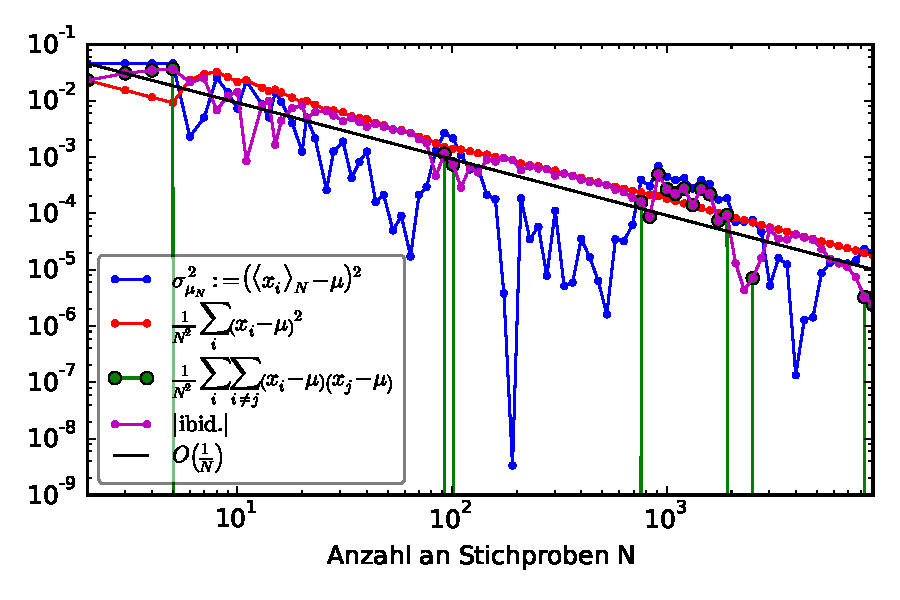
\includegraphics[width=\linewidth]{meanerror.pdf}
	\end{minipage}
	\caption{Darstellung der Standardvarianz des Mittelwertes $\sigma_{\mu_N}^2$ und der beiden in der Herleitung~\ref{eq:EabToEaEb-pre} auftretenden Summanden über die Anzahl einbezogener Stichproben. Hierbei ist zu beachten, dass beim Vergleich von den Werten für die Stichprobenanzahl von $N_1$ und $N_2$ die ersten $\min\left( N_1,N_2 \right)$ Stichproben identisch sind.}
	\label{fig:meanerrorsummand}
\end{figure}


%%%%%%%%%%%%%%%%%%%%%%%%%%%%%%%%%%%%%%%%%%%%%%%%%%%%%%%%%%%%%%%%%%%%%%%%%%%%%%%%%
%\chapter{Programmausdrucke}
%%%%%%%%%%%%%%%%%%%%%%%%%%%%%%%%%%%%%%%%%%%%%%%%%%%%%%%%%%%%%%%%%%%%%%%%%%%%%%%%%
%
%\lstinputlisting[language=bash, inputencoding=latin1, frame=single, caption={\lstinline!start_spark_slurm.sh! enthält Parameter für \lstinline!sbatch!, berechnet nötige Parameter für Spark aus denen von Slurm und startet dann einen Master und mehrere Worker-Prozesse startet}, label=lst:start_spark_slurm.sh]{../common/start_spark_slurm.sh}
%
%\lstinputlisting[language=bash, inputencoding=latin1, frame=single, caption={\lstinline!startSpark.sh! welche eine Funktion definiert die einen den Sparkslurmjob aus Listing~\ref{lst:start_spark_slurm.sh} startet und Master-IP aus der Logdatei extrahiert}, label=lst:startSpark]{../startSpark.sh}

%\begin{lstlisting}[language=C++,firstnumber=10, caption={Die Trapezregel wie in Formel~\ref{eq:trapeze}}, label=lst:trapezregel]
%    for (uint64_t i=1; i<N-1; i++)
%    {
%    (!!!)
%     dx + f(b);
%\end{lstlisting}\end{minipage}\end{center}

%\begin{eqnarray}
%	\label{eq:n}
%	 a = b
%\end{eqnarray}
%
%\begin{figure}
%	\centering
%	\begin{minipage}{0.7 \linewidth}
%		\includegraphics[width=\linewidth]{Image.pdf}
%	\end{minipage}
%	\caption{captiontext}
%	\label{fig:RTn}
%\end{figure}


% add image(s) on one line without figure-environment, to place it exactly where you want
%\begin{minipage}{\linewidth}\begin{center}\bigskip
%	\captionsetup{type=figure}
%	\begin{minipage}{0.45 \linewidth}
%		\includegraphics[width=\linewidth]{ImageLeft.pdf}
%	\end{minipage}
%	\begin{minipage}{0.45 \linewidth}
%		\includegraphics[width=\linewidth]{ImageRight.pdf}
%	\end{minipage}
%	\captionof{figure}{...}
%	\label{fig:figlabel}
%\bigskip\end{center}\end{minipage}

\end{document}


% Typical problem words of me:
%  - versuchen
%  - zig
%  - hierfür, hierbei
%  - komma for 'um + inifinitiv' vergessen
%  -

